% Options for packages loaded elsewhere
\PassOptionsToPackage{unicode}{hyperref}
\PassOptionsToPackage{hyphens}{url}
%
\documentclass[
]{book}
\usepackage{amsmath,amssymb}
\usepackage{iftex}
\ifPDFTeX
  \usepackage[T1]{fontenc}
  \usepackage[utf8]{inputenc}
  \usepackage{textcomp} % provide euro and other symbols
\else % if luatex or xetex
  \usepackage{unicode-math} % this also loads fontspec
  \defaultfontfeatures{Scale=MatchLowercase}
  \defaultfontfeatures[\rmfamily]{Ligatures=TeX,Scale=1}
\fi
\usepackage{lmodern}
\ifPDFTeX\else
  % xetex/luatex font selection
\fi
% Use upquote if available, for straight quotes in verbatim environments
\IfFileExists{upquote.sty}{\usepackage{upquote}}{}
\IfFileExists{microtype.sty}{% use microtype if available
  \usepackage[]{microtype}
  \UseMicrotypeSet[protrusion]{basicmath} % disable protrusion for tt fonts
}{}
\makeatletter
\@ifundefined{KOMAClassName}{% if non-KOMA class
  \IfFileExists{parskip.sty}{%
    \usepackage{parskip}
  }{% else
    \setlength{\parindent}{0pt}
    \setlength{\parskip}{6pt plus 2pt minus 1pt}}
}{% if KOMA class
  \KOMAoptions{parskip=half}}
\makeatother
\usepackage{xcolor}
\usepackage{longtable,booktabs,array}
\usepackage{calc} % for calculating minipage widths
% Correct order of tables after \paragraph or \subparagraph
\usepackage{etoolbox}
\makeatletter
\patchcmd\longtable{\par}{\if@noskipsec\mbox{}\fi\par}{}{}
\makeatother
% Allow footnotes in longtable head/foot
\IfFileExists{footnotehyper.sty}{\usepackage{footnotehyper}}{\usepackage{footnote}}
\makesavenoteenv{longtable}
\usepackage{graphicx}
\makeatletter
\def\maxwidth{\ifdim\Gin@nat@width>\linewidth\linewidth\else\Gin@nat@width\fi}
\def\maxheight{\ifdim\Gin@nat@height>\textheight\textheight\else\Gin@nat@height\fi}
\makeatother
% Scale images if necessary, so that they will not overflow the page
% margins by default, and it is still possible to overwrite the defaults
% using explicit options in \includegraphics[width, height, ...]{}
\setkeys{Gin}{width=\maxwidth,height=\maxheight,keepaspectratio}
% Set default figure placement to htbp
\makeatletter
\def\fps@figure{htbp}
\makeatother
\setlength{\emergencystretch}{3em} % prevent overfull lines
\providecommand{\tightlist}{%
  \setlength{\itemsep}{0pt}\setlength{\parskip}{0pt}}
\setcounter{secnumdepth}{5}
\usepackage{booktabs}
\ifLuaTeX
  \usepackage{selnolig}  % disable illegal ligatures
\fi
\usepackage[]{natbib}
\bibliographystyle{plainnat}
\usepackage{bookmark}
\IfFileExists{xurl.sty}{\usepackage{xurl}}{} % add URL line breaks if available
\urlstyle{same}
\hypersetup{
  pdftitle={MA132: Foundations Lecture Notes},
  pdfauthor={Jo Evans},
  hidelinks,
  pdfcreator={LaTeX via pandoc}}

\title{MA132: Foundations Lecture Notes}
\author{Jo Evans}
\date{2024-10-01}

\usepackage{amsthm}
\newtheorem{theorem}{Theorem}[chapter]
\newtheorem{lemma}{Lemma}[chapter]
\newtheorem{corollary}{Corollary}[chapter]
\newtheorem{proposition}{Proposition}[chapter]
\newtheorem{conjecture}{Conjecture}[chapter]
\theoremstyle{definition}
\newtheorem{definition}{Definition}[chapter]
\theoremstyle{definition}
\newtheorem{example}{Example}[chapter]
\theoremstyle{definition}
\newtheorem{exercise}{Exercise}[chapter]
\theoremstyle{definition}
\newtheorem{hypothesis}{Hypothesis}[chapter]
\theoremstyle{remark}
\newtheorem*{remark}{Remark}
\newtheorem*{solution}{Solution}
\begin{document}
\maketitle

{
\setcounter{tocdepth}{1}
\tableofcontents
}
\chapter{About}\label{about}

These are the 2024-25 lecture course for the Warwick undergraduate course MA132: Foundations. The material up to chapter 7 is also relevant to joint degree students taking Sets and Numbers.

These notes are heavily based on previous notes of Saul Schleimer and Dave Wood, though all mistakes are my own!

Please send me any typos (or possible typos) that you find. And be on the look out for typos.

\section{How to use these notes}\label{how-to-use-these-notes}

These notes are designed to generate both a html version (which should work well with screen readers) and a latex generated pdf and epub (which will work better if you want to print the notes). You can access the pdf/epub by pressing the download button in the top right (little down arrow).

Everything you need to know for the exam and future courses should be contained in these notes. There will also be examples, some discussions and some non-examinable sections.

Similarly, almost everything you need to know will be written by me on the board in lectures. There may be some exceptions which I will warn you about!

There are three main ways that undergraduates typically use printed lecture notes:

\begin{enumerate}
\def\labelenumi{\arabic{enumi}.}
\item
  They take their own notes during the lecture (or take none) and refer to these notes outside the lecture to supplement those notes, to check things, when doing exercises, or during revision.
\item
  They print out a copy of these notes/or have them available as a pdf on a tablet and annotate them during the lectures.
\item
  They take a copy of these notes to lectures to refer to but don't annotate them.
\end{enumerate}

\chapter{Sets and Functions}\label{sets-and-functions}

\section{What is a set?}\label{what-is-a-set}

We begin with sets which are one of the basic objects of mathematics. Set theory becomes very complicated very quickly when you begin to explore the subtleties. We will discuss some of the pitfalls and paradoxes in a non-examinable section later but first we focus on when things are simple.

\begin{definition}[set]
A \emph{set} is a collection of mathematical objects.
\end{definition}

To make sense of this definition we need to consider some examples of things that are and are not sets.

\begin{example}
The function \(y = x^2, x \in \mathbb{R}\) is \emph{not} a set (it's a function as we wrote). However we can form a \emph{set} of the form \[ \{(x,y)\,:\,  x \in \mathbb{R}, y \in \mathbb{R}, y=x^2 \}.  \]
\end{example}

\begin{example}
The natural numbers \(\mathbb{N} = \{0,1,2, 3, 4, \dots\}\) is a set. We can see in this and the previous example that you can often recognise sets because they have curly brackets around them. However, this is not foolproof. We can write this set as \(\mathbb{N}\) and there are no curly brackets.

If you haven't seen it before remember this notation for the natural numbers. It will come up a lot!

This example also has another bit of common mathematical notation in its. The set of three dots at the end of the sequence of numbers. This indicates that the sequence will continue as you would expect it to.
\end{example}

\begin{example}
Sets can also have a finite number of elements. For example the following set \(\{12\}\) which contains only the integer 12. As with the first example with a function, we make a distinction between the object which is the integer 12 and a set that contains only the integer 12.
\end{example}

\begin{example}
All the examples of sets above involve mathematical objects which are numbers (or pairs of numbers in the first example). We aren't limited to this. We might consider the set of all polynomials with integer coefficients (where all the elements are functions) or the set of all sequences of real numbers tending to zero (where all the elements are sequences). You can also consider sets with a mixture of different types of elements. e.g.~
\[ \{ 4, (\pi, \pi^2), \{1/n \,:\, n \in \mathbb{N}, n \neq 0 \}, \mbox{the function}\, f(x) = x^2\}.  \] Here notice that one of the elements of this set is a set itself. This is perfectly possible.
\end{example}

We need to be able to talk and write about sets. We often give sets names (usually a letter) and we write

\[ A = \{1,2,7\}.  \]

We then want to be able to say whether something is or isn't in the set so we write
\[ 1 \in A  \] to mean \(1\) is in the set \(A\) or \(1\) is an element of the set \(A\). We also write
\[ 3 \notin A \] to mean that \(3\) is not an element of the set \(A\) or that 3 isn't in \(A\).

\begin{definition}

There are some important sets which have their own symbols and names. You have probably met them before:

\begin{itemize}
\item
  The natural numbers, \(\mathbb{N}= \{0, 1,2,3,\dots\}\),
\item
  The integers, \(\mathbb{Z} = \{ \dots, -3, -2, -1, 0, 1, 2, 3, \dots \}\),
\item
  The rationals, \(\mathbb{Q} = \{p/q \,:\, p \in \mathbb{Z}, q \in \mathbb{N}\}\),
\item
  The real numbers, \(\mathbb{R} = (-\infty, \infty)\),
\item
  The complex numbers, \(\mathbb{C} = \{x+iy \,:\, x \in \mathbb{R}, y \in \mathbb{R}\}\) where \(i\) is the complex unit.
\item
  Something that will appear in this course \([[n]]= \{0,1,\dots, n-1\}\).
\end{itemize}

\end{definition}

\begin{definition}[equality of sets/axiom of extension]
Two sets are equal (the same) if they have exactly the same elements. We call this the axiom of extension. We can write it in formal language as: if for every \(x \in A\) we have \(x \in B\) and for every \(y \in B\) we have \(y \in A\) then \(A=B\).
\end{definition}

\begin{remark}
It might seem obvious at this point that any two sets with the same element are the same. However there are two important ways this comes up.

In a proof we might write a set in two very different ways for example \([0,\infty) = \{ x \in \mathbb{R} \,:\, \mbox{there exists}\, y \in \mathbb{R}\, \mbox{s.t.} y^2 = x\}\).

We might end up writing a set in a way that means some element appears in the representation multiple times e.g.~\(\{0\}\) and \(\{0, 0\}\). The axiom of extension makes it clear that these are both the same set. It also tells us that there aren't multiple different sets containing only the element \(0\) there is just one the set \(\{0\}\).
\end{remark}

At this point it is useful to introduce some notation that you may or may not have seen before. We will talk about this notation more thoroughly in the section on proof. In my opinion it is useful to see all this notation a bit before we think about it too thoroughly.

\begin{definition}
There are several shorthand notations used in maths and particularly in logic. Some are more common than others and it is always okay and often wise not to overuse symbols. We might use the following:

-We use the symbol \(\forall\) as a shorthand for the phrase \emph{for every} or \emph{for all}.

-We use the symbol \(\exists\) to mean \emph{there exists} or \emph{there is at least one}.

-We use the symbol \(\Rightarrow\) to mean \emph{implies} and (much less often) the symbol \(\Leftarrow\) to mean \emph{is implied by}.

-We use the symbol \(\Leftrightarrow\) to mean \emph{if and only if} which we also sometimes abbreviate to iff. If and only if is a common phrase in pure maths but it might sometimes be easier to say \emph{exactly when} to mean the same thing.
\end{definition}

Using this we can write the axiom of extension as
\[ \forall A \forall B ( \forall x (x \in A \Leftrightarrow x \in B) \Rightarrow (A=B)).   \] Which is a good illustration of why its often better to use words!

Given that sets are defined by their elements we sometimes need to consider that set that doesn't have any elements at all.

\begin{definition}[the empty set (Axiom)]
There exists a set which contains no elements. We call this the \emph{empty set} and write it with the symbol \(\emptyset\).
\end{definition}

\begin{remark}
Here if you've been paying attention you'll notice that \(\emptyset \neq \{\emptyset\}\). The first contains no elements, the second contains one element which is the empty set. You can also have \(\{\emptyset, \{\emptyset\}\}\) and \(\{\emptyset, \{\emptyset\}, \{\{\emptyset\}\}\}\) and so on if you would like to reassure yourself that there exists a set containing \(k\) elements for any \(k \in \mathbb{N}\) but you are unconvinced of the existence of the natural numbers. (If you are in this position you might be Bertrand Russell.)
\end{remark}

\section{Subsets}\label{subsets}

You might be interested in looking at only part of a set. This is called a subset.

\begin{definition}[Subset]

If \(A\) and \(B\) are sets and for every \(x \in A\) we have that \(x \in B\) then we say \(A\) is a \emph{subset} of \(B\) which we write
\[ A \subset B.  \]

\begin{figure}
\centering
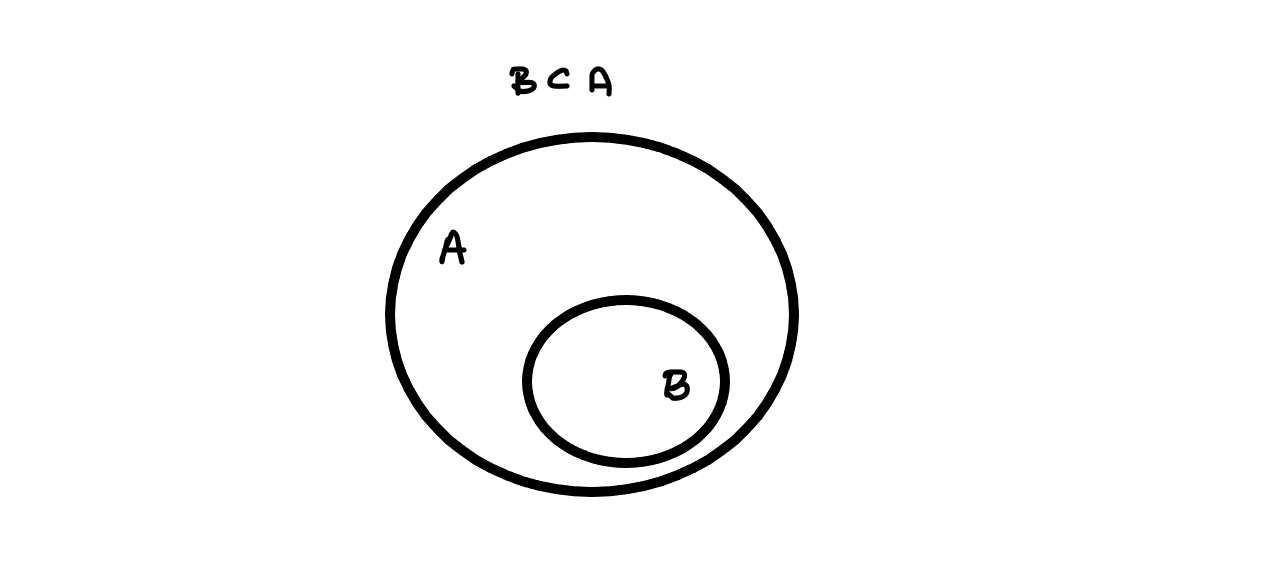
\includegraphics{subset.png}
\caption{\label{fig:unnamed-chunk-1}Picture showing A as a subset of B with sets indicated by circles}
\end{figure}

\end{definition}

\begin{example}

\begin{itemize}
\tightlist
\item
  \(1\) is \emph{not} a subset of \(\{1\}\).
\item
  The even numbers are a subset of \(\mathbb{N}\).
\item
  \(\{1\}\) is a subset of \(\mathbb{N}\).
\item
  \(\{1\}\) is \emph{not} a subset of \(\{\{1\}\}\).
\end{itemize}

\end{example}

\begin{remark}
Sometimes when you are writing you wish to specify the set and the subset in a different order. We write \(B \supset A\) and this expresses exactly the same information as \(A \subset B\). When we read the expression \(B \supset A\) we say \(B\) contains \(A\) or \(B\) is a superset of \(A\).
\end{remark}

The following is also always true

\begin{lemma}

For any set \(A\) we have

\begin{itemize}
\item
  \(\emptyset \subset A\),
\item
  \(A \subset A\)
\end{itemize}

\end{lemma}

\begin{proof}
Remember to show that \(B \subset A\) we need to show that for every \(y \in B\) we have that \(y \in A\).

For the first statement since there are no elements of the empty set so absolutely any statement about every element of the empty set is true.

For the second statement if \(x \in A\) then tautologically \(x \in A\) so we have \(A \subset A\).
\end{proof}

Following from this we have

\begin{lemma}

For two sets \(A, B\) the following are equivalent:

\begin{enumerate}
\def\labelenumi{\arabic{enumi}.}
\item
  \(A = B\),
\item
  \(A \subset B\) and \(B \subset A\).
\end{enumerate}

\end{lemma}

\begin{proof}
Exercise!
\end{proof}

\begin{definition}
We call a set which contains only one element a \emph{singleton set}.
\end{definition}

\section{Power sets and specification}\label{power-sets-and-specification}

\begin{definition}[Power set (axiom)]
Given a set \(A\) there exists another set \(\mathcal{P}(A)\) called the \emph{power set} of \(A\) which is the set of all possible subsets of \(A\).
\end{definition}

\begin{example}
The power set of \(\{0,1,2\}\) is
\[ \{ \emptyset, \{0\}, \{1\}, \{2\}, \{0,1\}, \{0,2\}, \{1,2\}, \{0,1,2\}\}.  \]
\end{example}

\begin{definition}[specification (axiom)]
\emph{Specification} is a way of constructing subsets of a set (we've done this a lot already). Suppose \(P(A)\) is a property that an element \(x\) of \(A\) could have. Then we can define the set
\[ B = \{ x \in A \,:\, P(x)\}.  \]
\end{definition}

The \emph{axiom of specification} is the set theory axiom positing that such a set exists. In this we would need a more precise notion of what a property is.

\begin{example}
The very first set we defined was defined using specification
\[ \{(x, y)\,:\, x \in \mathbb{R}, y \in \mathbb{R}, y=x^2\}.  \]
\end{example}

\section{Functions}\label{functions}

\begin{definition}[function]
A function is comprised of three objects, a domain \(A\) which is a set, a co-domain \(B\) which is another set and a rule \(f\) which assigns an element \(f(x) \in B\) to each element \(x\) of \(A\).

We write \(f: A \rightarrow B\).
\end{definition}

\begin{remark}
This is a slightly informal definition. This is because we don't want to create an axiom saying functions exist. We are going to build functions out of more fundamental objects soon but first we want to have a useable definition.
\end{remark}

\begin{example}
\(f(x) = x^2 : \mathbb{R} \rightarrow \mathbb{R}\) is a function and technically \(f(x) = x^2: \mathbb{R} \rightarrow [0,\infty)\) is a different function.
\end{example}

A function can only take one value so we have to be careful when dealing with things like square roots. Similarly a function needs to take exactly one value so we also need to make sure it is defined everywhere.

\begin{definition}
If \(f: A \rightarrow B\) is a function then if \(y = f(x)\) we call \(y\) the \emph{image} of \(x\) under \(f\). We also call \(x\) a \emph{preimage} of \(y\) under \(f\).

Notice that an element of \(X\) can have only one image but an element of \(Y\) can have multiple or zero preimages.
\end{definition}

\begin{definition}
The identity function on \(A\) is written \(Id_A : A \rightarrow A\) and is defined by \(Id_A(x)=x\).
\end{definition}

\begin{definition}[restriction to a subset]
Suppose that \(A\) and \(B\) are sets and \(f : A \rightarrow B\) is a function, and suppose further that \(C \subset A\). Then we can define a new function called the restriction of \(f\) to \(C\) which we write \(f|_C\). This is a function with domain \(C\) and codomain \(B\) and for \(x \in C\) we have \(f|_C(x) = f(x)\).
\end{definition}

\begin{definition}[Indicator function]
Given a set \(A\) and a subset \(B \subset A\) we can define the indicator function of \(B\), from \(A\) to \(\{0,1\}\) by
\[ 1_B(x) = \left\{\begin{array}{cc} 0 & x \not\in B\\ 1 & x \in B \end{array} \right. \]
\end{definition}

\begin{definition}[image and pre-image]

Given a function \(f:A \rightarrow B\) then

\begin{itemize}
\item
  If \(C \subset A\) we write \(f(C) = \{y \in B \,:\, y = f(x) \, \mbox{for some} \, x \in C\}\). We call \(f(C)\) the \emph{image} of \(C\) under \(f\).
\item
  If \(D \subset B\) we write \(f^{-1}(D) = \{ x \in A \,:\, f(x) \in D\}\). We call \(f^{-1}(D)\) the \emph{pre-image} of \(D\) under \(f\).
\end{itemize}

\end{definition}

\begin{example}
We have to be particularly careful with preimages as this example demonstrates

Let \(f: \mathbb{R} \rightarrow \mathbb{R}\) given by \(f(x) = x^2\) then \(f^{-1}(\{2\}) = \{-\sqrt{2}, \sqrt{2}\}\).

Let \(f: \mathbb{Q} \rightarrow \mathbb{Q}\) given by \(f(x) = x^2\) then \(f^{-1}(\{2\})= \emptyset\). Because \(\pm sqrt{2}\) is irrational so \(2\) has no square roots in the rationals.

Let \(f: [0, \infty) \rightarrow [0, \infty)\) given by \(f(x)=x^2\) then \(f^{-1}(\{2\}) = \{\sqrt{2}\}\).
\end{example}

\section{Properties of functions}\label{properties-of-functions}

\begin{definition}[injectivity]
A function \(f:A\rightarrow B\) is called \emph{injective} if \(f(x)=f(x')\) implies that \(x=x'\). That is to say there are no two elements of \(A\) where \(f(x)\) takes the same value, or \(y\) has at most one preimage under \(f\).
\end{definition}

\begin{example}
The function \(f: \mathbb{R} \rightarrow \mathbb{R}\) defined by \(f(x) =x^2\) is not injective because for every \(y>0\) there are two possible values of \(x\) such that \(x^2 = y\).

However, the function \(f: [0, \infty) \rightarrow \mathbb{R}\) is injective because now for every \(y\geq 0\) there is exactly one \(x\) such that \(x^2=y\) and for every \(y <0\) there are no elements \(x\) in the set such that \(x^2 = y\) (so for any \(y\) in the codomain there is never more than one element \(x\) in the domain so that \(x^2 = y\)).
\end{example}

\begin{figure}
\centering
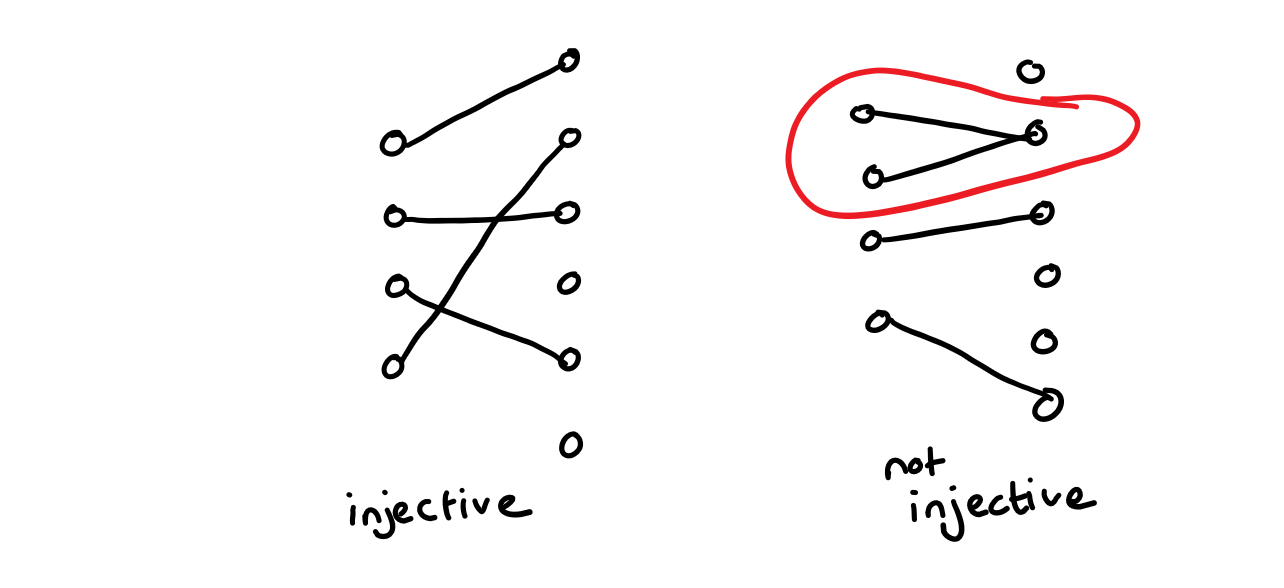
\includegraphics{injective.png}
\caption{\label{fig:unnamed-chunk-2}example of an injective function}
\end{figure}

\begin{definition}[surjectivity]
A function \(f: A \rightarrow B\) is called \emph{surjective} if for every \(y \in B\) there exists \(x \in A\) with \(f(x)=y\). That is to say the function \(f\) hits every element of the set \(B\) or that \(y\) has at least one preimage under \(x\).
\end{definition}

\begin{example}
The function \(f:\mathbb{R} \rightarrow \mathbb{R}\) defined by \(f(x) = x^2\) is not surjective because for \(y<0\) there is no element \(x\) of the domain so that \(x^2=y\).

However, the function \(f: \mathbb{R} \rightarrow [0,\infty)\) is surjective because for every element \(y\) of the codomain we have some \(x\) in the domain with \(x^2 =y\).
\end{example}

\begin{figure}
\centering
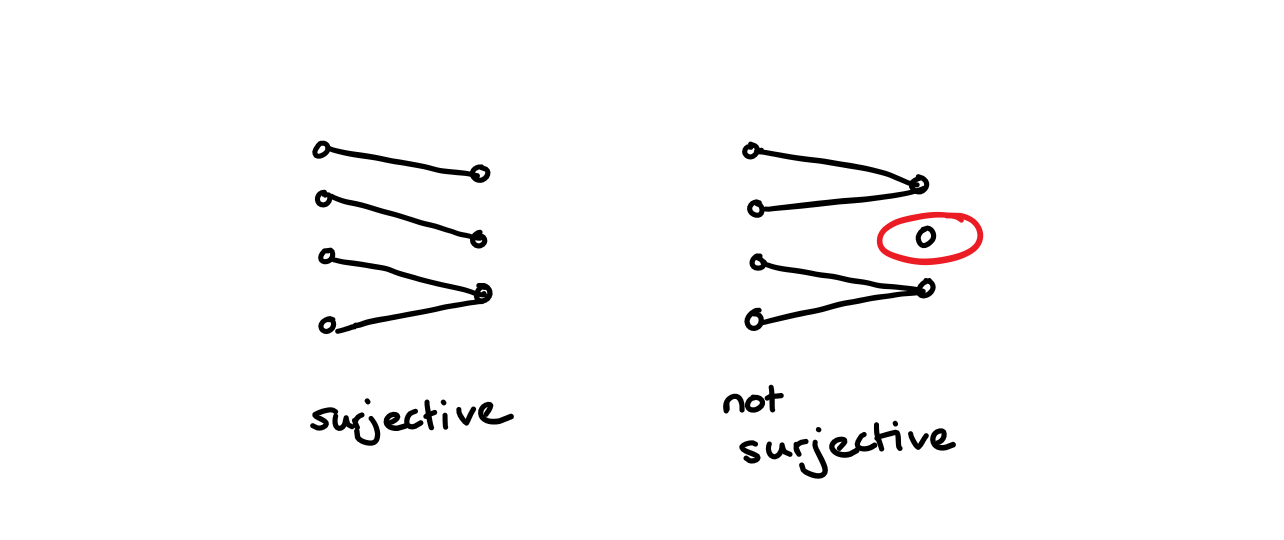
\includegraphics{surjective.png}
\caption{\label{fig:unnamed-chunk-3}example of a surjective function}
\end{figure}

\begin{definition}[bijectivity]
A function is called \emph{bijective} if it is both \emph{surjective} and \emph{injective}.
\end{definition}

\begin{remark}
Bijective functions are often called matchings because if \(f: A \rightarrow B\) is a bijection then we \emph{match} every element of \(A\) with an element of \(B\).
\end{remark}

\begin{figure}
\centering
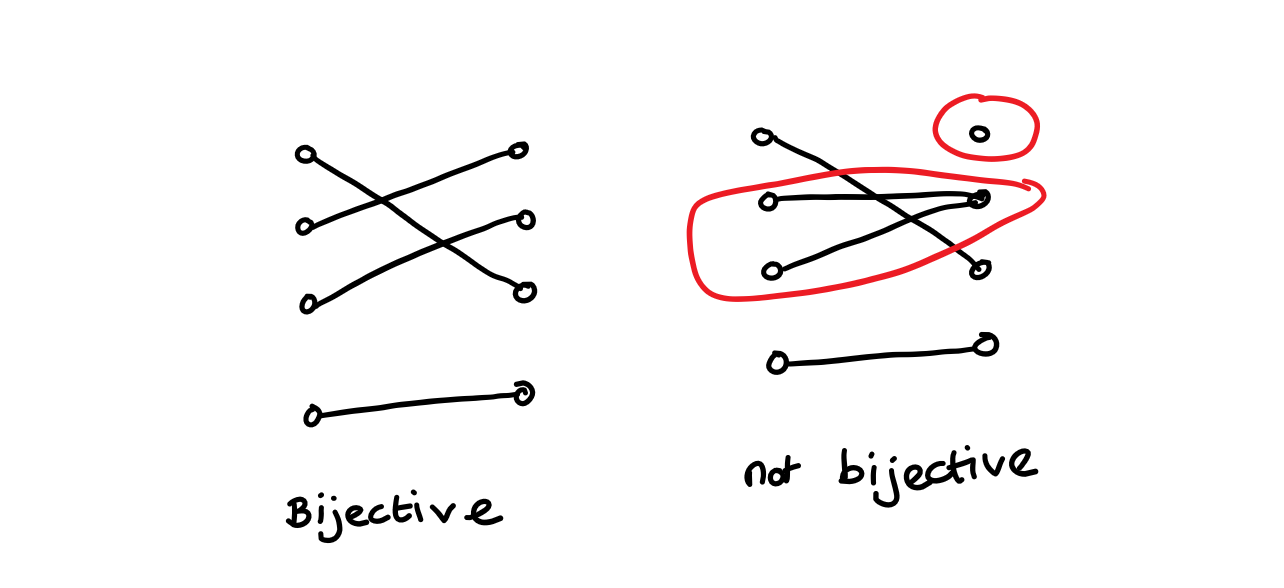
\includegraphics{bijective.png}
\caption{\label{fig:unnamed-chunk-4}example of a bijective function}
\end{figure}

\section{Cardinality}\label{cardinality}

If \(f: A \rightarrow B\) is a bijection then that tells us something important about the relationship between \(A\) and \(B\).

\begin{definition}[Cardinality]
We say that \(A\) and \(B\) have the same \emph{cardinality} (informally the same size) if there exists a bijection between \(A\) and \(B\). We often write \(|A| = |B|\).
\end{definition}

\begin{definition}[Finiteness]
Cardinality allows us to give a rigorous notion for a set to be \emph{finite}/have a finite number of elements.

Given a set \(A\), if there is some natural number \(n\) such that \(|A|=|[[n]]|\) then we say \(A\) has size \(n\).

If \(A\) has size \(n\) for some \(n\) then we say \(A\) is finite.
\end{definition}

\begin{definition}[infinite]
We say a set is \emph{infinite} if it isn't finite.
\end{definition}

\begin{theorem}[Cantor's Theorem]
Let \(A\) be a set and \(f: A \rightarrow \mathcal{P}(A)\) then \(f\) cannot be a surjection.

You could also say: there is no surjection between a set and its power set.
\end{theorem}

\begin{remark}
One implication of this theorem is that a set cannot be the same size as its power set. This is obvious for finite sets; if \(|A|=n\) then \(|\mathcal{P}(A)|= 2^n\) but it isn't clear for infinite sets.
\end{remark}

\begin{proof}
We notice that for every \(x \in A\) we have \(f(x)\) which is a subset of \(A\). This brings up two possibilities we could have \(x \in f(x)\) or \(x \notin f(x)\). We can form a set \(C\) by writing
\[ C = \{ x \in A\,:\, x \notin f(x)\}.  \]

Now suppose for contradiction that \(f\) is surjective. This implies that there exists some \(c \in A\) such that \(f(c) = C\).

Now there are two possibilities.

\begin{enumerate}
\def\labelenumi{\arabic{enumi}.}
\item
  \(c \in C\) which is a contradiction because we defined \(C\) to be the set of \(x\) for which \(x \notin f(x)\).
\item
  \(c \notin C\) which is also a contradiction because then if \(C\) is the set of all \(x\) for which \(x \notin f(x)\) so should contain \(c\).
\end{enumerate}

Therefore we have a contradiction to \(f\) being surjective.
\end{proof}

\begin{figure}
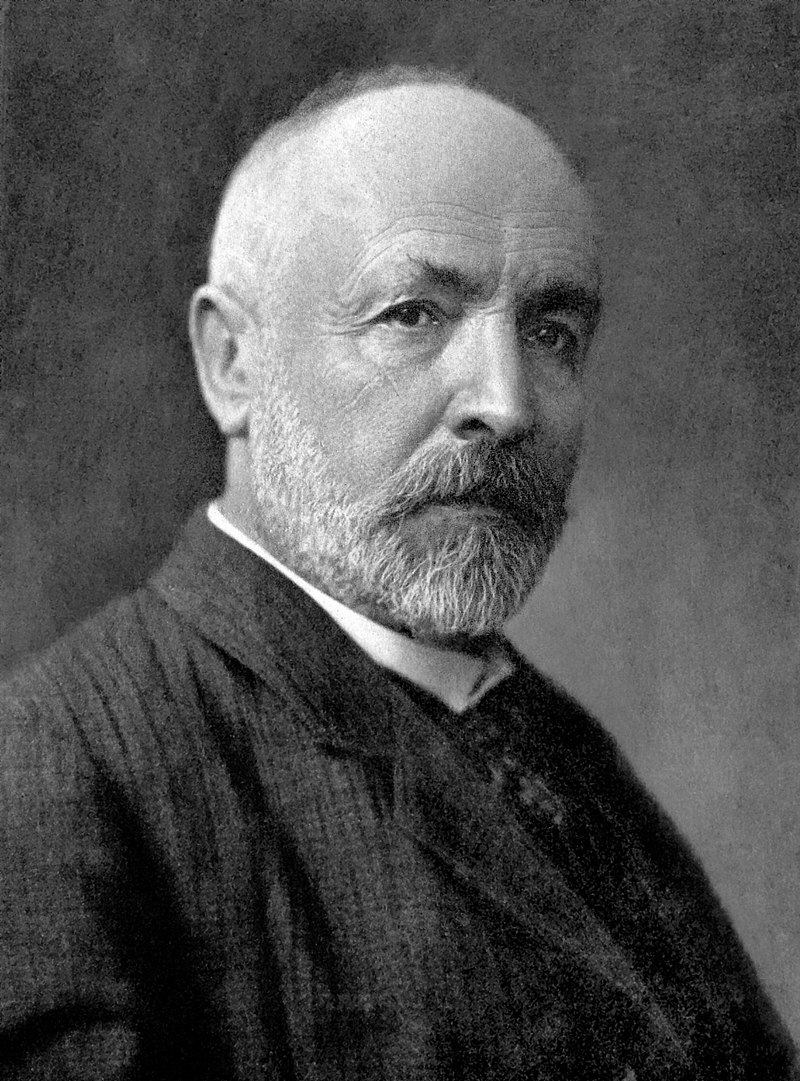
\includegraphics[width=0.3\linewidth]{Cantor} \caption{A picture of Cantor}\label{fig:unnamed-chunk-5}
\end{figure}

Cantor was one of the pioneers of the foundations of mathematics and in particular set theory. His work was astonishingly controversial at the time. One of the implications of Cantor's theorem which we haven't explored is the existence of an infinity which is \emph{larger} in some sense than the infinity that is the cardinality of the natural numbers. Some theologians believed this as a step towards pantheism. He was also described as a ``corrupter of youth''.

\begin{remark}[non-examinable]
The proof of Cantor's theorem is is strongly related to *Russel's paradox''. Let us consider the set \(R= \{ \mbox{all sets}\, x \,\mbox{such that} \, x \notin x \}\) then the question is whether \(R \in R\)?

It becomes clear from this that we cannot define the set \(R\) so we do not want to build an axiom set which would allow us to define something like \(R\).
\end{remark}

\section{Ordered pairs and Cartesian products}\label{ordered-pairs-and-cartesian-products}

When we think about functions we often think about the graph of a function. Therefore is is useful to enhance our set theory in a way that allows us to talk about graphs.

\begin{definition}[ordered pairs]
If we have two sets \(X\) and \(Y\) and \(x \in X, y \in Y\) then we can form an ordered pair of these two elements that we write \((x,y)\).
\end{definition}

\begin{remark}
Here we say \emph{ordered} pair because the order matters. So \((1,2) \neq (2,1)\). This is different to how sets behave where \(\{1,2\} = \{2,1\}\). Also unlike setes we keep repeats. We can have a pair \(x,x\) if \(x \in X\) and \(x \in Y\) and this is different to the element \(x\).
\end{remark}

\begin{definition}[cartesian product]
Given two sets \(X\) and \(Y\) we can form a new set \(X \times Y\) called the \emph{Cartesian product} of \(X\) and \(Y\) and defined by
\[ X \times Y = \{ (x,y) \,:\, x \in X, y \in Y\}.  \]
\end{definition}

\begin{remark}
We have a special notation for the Cartesian product between a set and itself. We write
\[ X^2 = X \times X,  \] and
\[ X^n = X \times X^{n-1}.  \] You will have probably seen this before e.g.~\(\mathbb{R}^d\).
\end{remark}

\section{Graphs and a better definition of functions}\label{graphs-and-a-better-definition-of-functions}

Relations are an important mathematical object that you might not have thought about before. At first they seem quite similar to functions but they can appear in a very different settings. Since this is a section a about functions we are just going to talk enough about relations to give a better definition of a function and then return to them later.

\begin{definition}[Graphical relations]
A \emph{graphical relation} is formed of three objects

\begin{itemize}
\item
  A domain \(X\)
\item
  A codomain \(Y\)
\item
  A subset \(G \subset X \times Y\) which saitsfies that for every \(x \in X\) there exists exactly one \(y \in Y\) such that \((x,y) \in G\).
\end{itemize}

If \((x,y) \in G\) we write \(xGy\).
\end{definition}

\begin{example}

The relation defined by \((x,y) \in G \Leftrightarrow x \leq y\) is not graphical from \(\mathbb{R}\) to itself because for every \(x\) there are many \(y\) with \(y \leq x\).

\begin{figure}
\centering
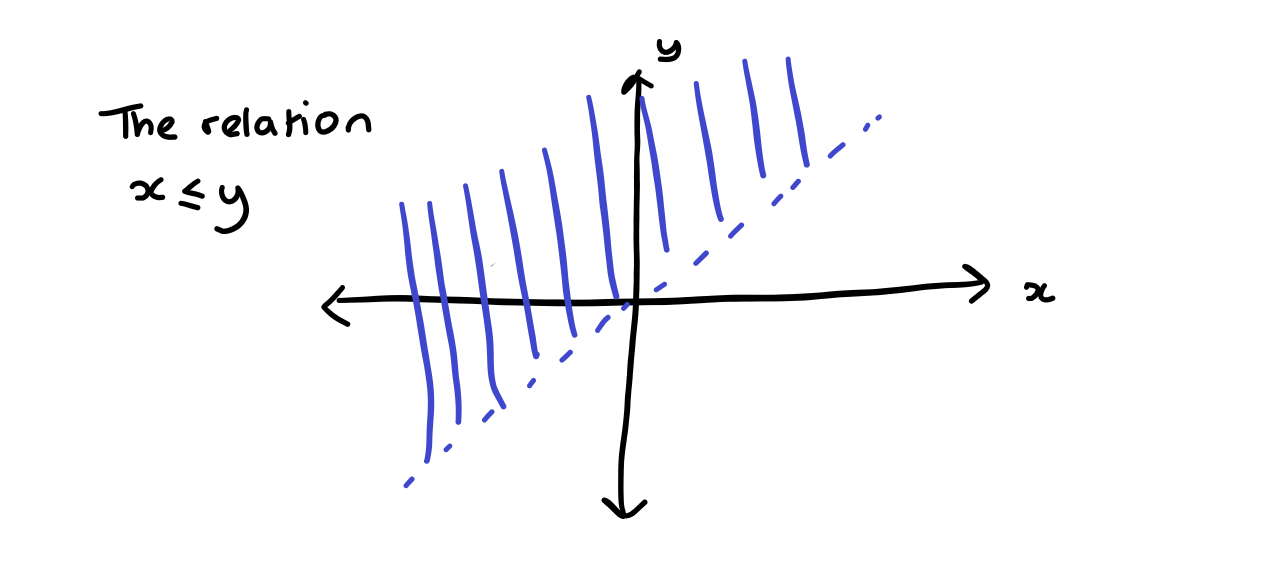
\includegraphics{less than.png}
\caption{\label{fig:unnamed-chunk-6}A picture of the less than relation on the reals}
\end{figure}

The relation defined by \((x,y) \in G \Leftrightarrow x=y^2\) is not graphical from \(\mathbb{R}\) to itself because if \(x\) is negative then it isn't the square of any real number so there are no \(y\)s with \(x G y\), and also because for \(x \geq 0\) there are two \(y\)s with \(x=y^2\).

\begin{figure}
\centering
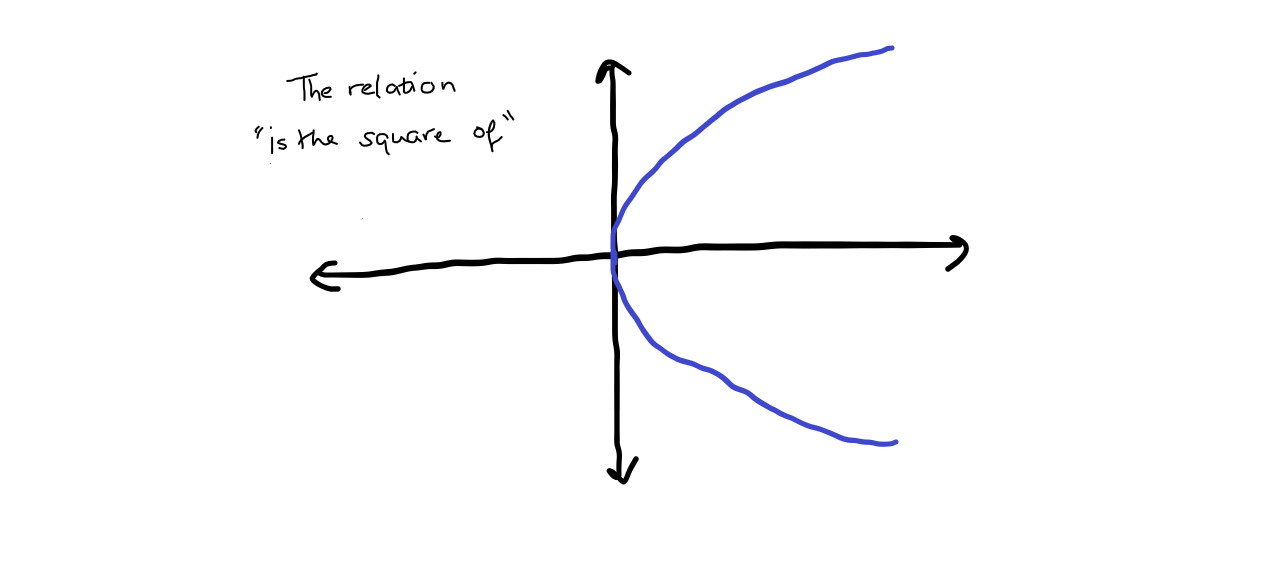
\includegraphics{is the square of.png}
\caption{\label{fig:unnamed-chunk-7}A picture of the is the square of relation}
\end{figure}

The relation defined by \((x,y) \in G \Leftrightarrow x=y^3\) on \(\mathbb{R}\) \emph{is} graphical because for every \(x \in \mathbb{R}\) there is exactly one \(y \in \mathbb{R}\) such that \(x=y^3\).

\begin{figure}
\centering
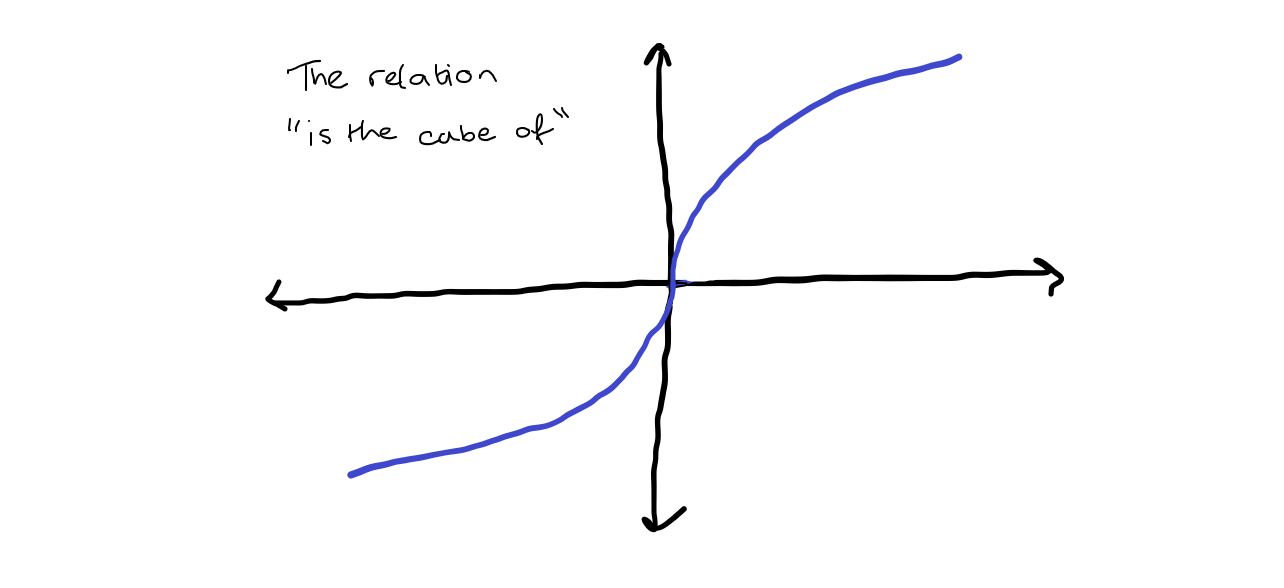
\includegraphics{is the cube of.png}
\caption{\label{fig:unnamed-chunk-8}A picture of the is the cube of relation}
\end{figure}

\end{example}

Using this we can give a better definition of a function

\begin{definition}[function]
Given a graphical relation \((x,Y,G)\) we can define a function \(f\) with domain \(X\) and co-domain \(Y\) by setting \(f(x) = y\) for the unique \(y\) such that \((x,y) \in G\).
\end{definition}

\begin{remark}
It is interesting \emph{and subtle} to think about why this is a more satisfactory definition of a function. People who worked on the foundations of mathematics wanted to build all mathematical objects from sets using a fairly small set of axioms.

We have done something in this direction, but starting only with sets and axioms it would take a very long time to define everything we need for this course. It is also challenging and not to everybodies taste. Here we have skipped some steps, hidden some subtleties, added axioms to make it simpler etc. For example, in the axiom of separation we have not really defined what we mean by a property, and we have used the natural numbers without defining them starting from sets.

Most of the time when we've introduced new axioms, we are asserting that some set exists (e.g.~a power set, union, etc.). If we wanted to add an axiom saying functions exist/make sense this would mean adding an axiom that doesn't just say ``another kind of set exists'' it would say ``a completely new kind of object exists'' and this is in some sense very unsatisfactory. Therefore, this later more formal definition of function is \emph{better} because it allows us to say what a function is using only concepts about sets and subsets.
\end{remark}

\chapter{Operations on sets and functions}\label{operations-on-sets-and-functions}

\section{Set operations}\label{set-operations}

We have already seen a few ways of making new sets from old like specification or taking Cartesian products. We are now going to look at some common \emph{set operations} which allow us to make lots of new sets.

\begin{definition}[union]
The union of two sets \(A\) and \(B\) is set containing all the elements that are in \(A\) or \(B\) (or both). We write it \(A\cup B\).

\begin{figure}
\centering
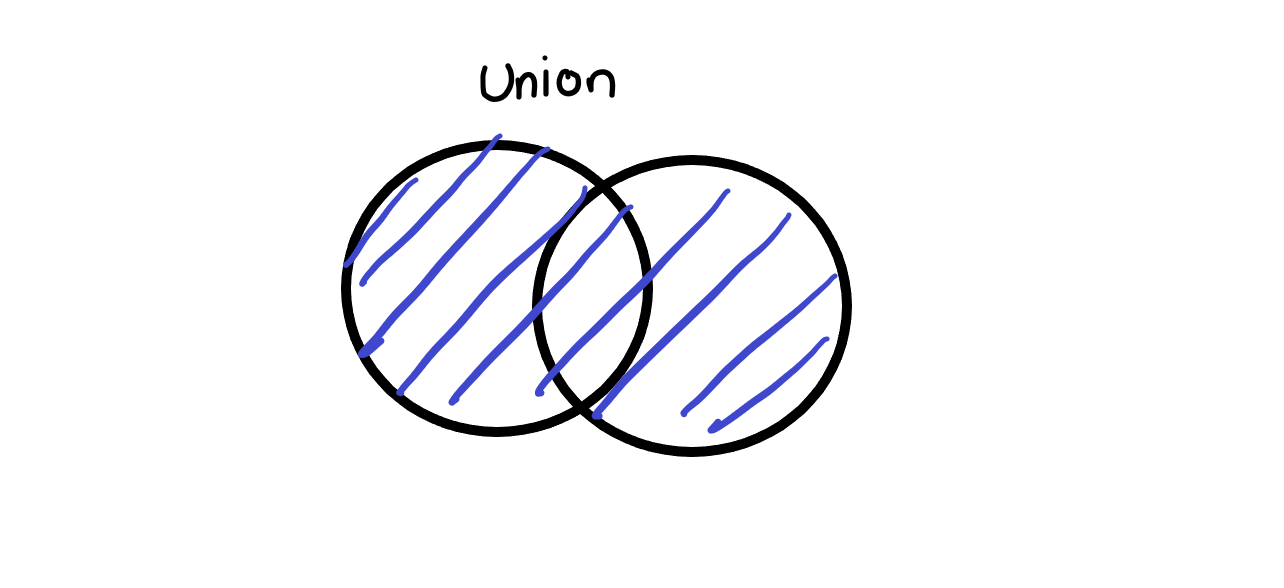
\includegraphics{union.png}
\caption{\label{fig:unnamed-chunk-9}picture of a union of two sets, sets represented as overlapping circles}
\end{figure}

We don't just have to take unions over pairs of sets. In fact we can take a union over almost any collection of sets. Formally, suppose that \(C\) is a set all of whose elements are sets then we can define a new set
\[ \bigcup C = \{ x \,:\, \exists S \in C\, \mbox{s.t.}\, x \in S\}.\]
\end{definition}

\begin{remark}
In practice most unions we take over larger collections of sets won't be written like they are in the formal definition. It is common so see a union taken of a sequence of sets \(A_1, A_2, A_3, \dots\) then we write \(\bigcup_n A_n\) to be the union of all these sets.
\end{remark}

\begin{example}
\[ \{1,2,3\} \cup \{ 1,2, 4\} = \{1,2,3,4\}.\]
\end{example}

\begin{example}
\[ \bigcup_{n \in \mathbb{N}} [[n]] = \mathbb{N}. \]
\end{example}

\begin{lemma}

Suppose that \(A, B\) and \(C\) are sets then the following are true

\begin{itemize}
\item
  \(A \cup \emptyset = A\),
\item
  \(A \cup (B \cup C) = (A \cup B)\cup C\),
\item
  \(A \cup B = B \cup A\),
\item
  \(A \cup B = B\) if and only if \(A \subseteq B\),
\item
  \(A \cup A = A\)
\end{itemize}

\end{lemma}

Another very important \emph{set operation} is taking intersections.

\begin{definition}[intersection]

Given two sets \(A\) and \(B\) the \emph{intersection} of \(A\) and \(B\) is the set containing the elements in \emph{both} \(A\) and \(B\).

\begin{figure}
\centering
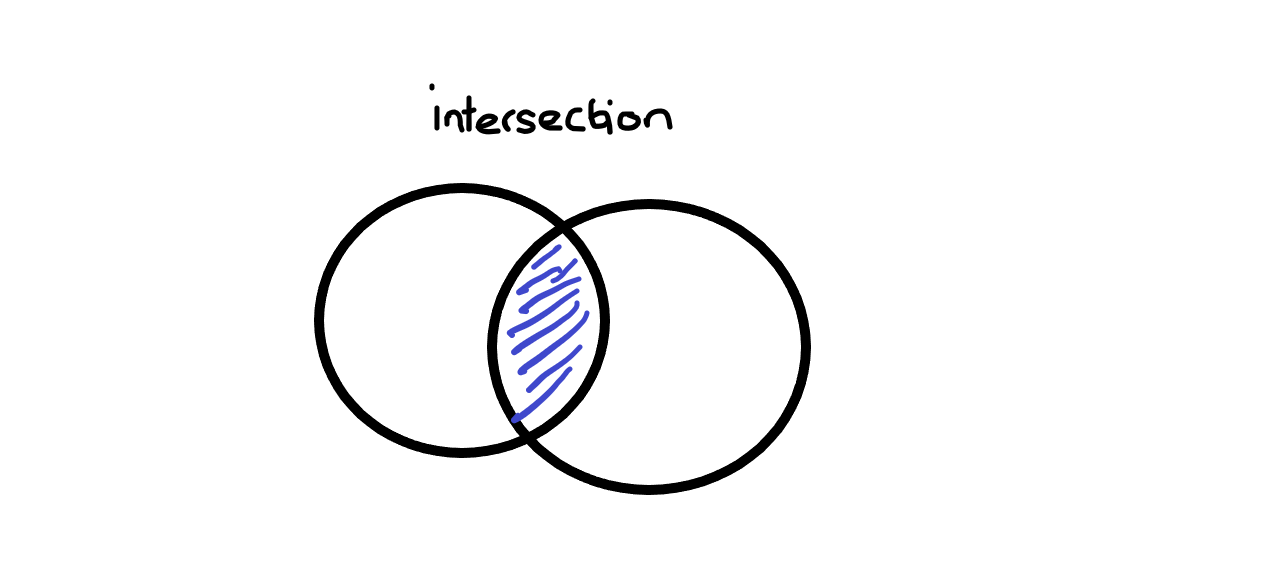
\includegraphics{intersection.png}
\caption{\label{fig:unnamed-chunk-10}picture of the intersection of two sets, sets represented by overlapping circles}
\end{figure}

As with unions, we don't have to do this with a pair of sets. If \(C\) is a set all of whose elements are sets we can write
\[ \bigcap C = \{ x \,:\,  x \in S \, \forall \, S \in C\}.  \]

An important piece of notation is that if \(A\) and \(B\) are sets with \(A \cap B = \emptyset\) then we say that \(A\) and \(B\) are \emph{disjoint}.

\begin{figure}
\centering
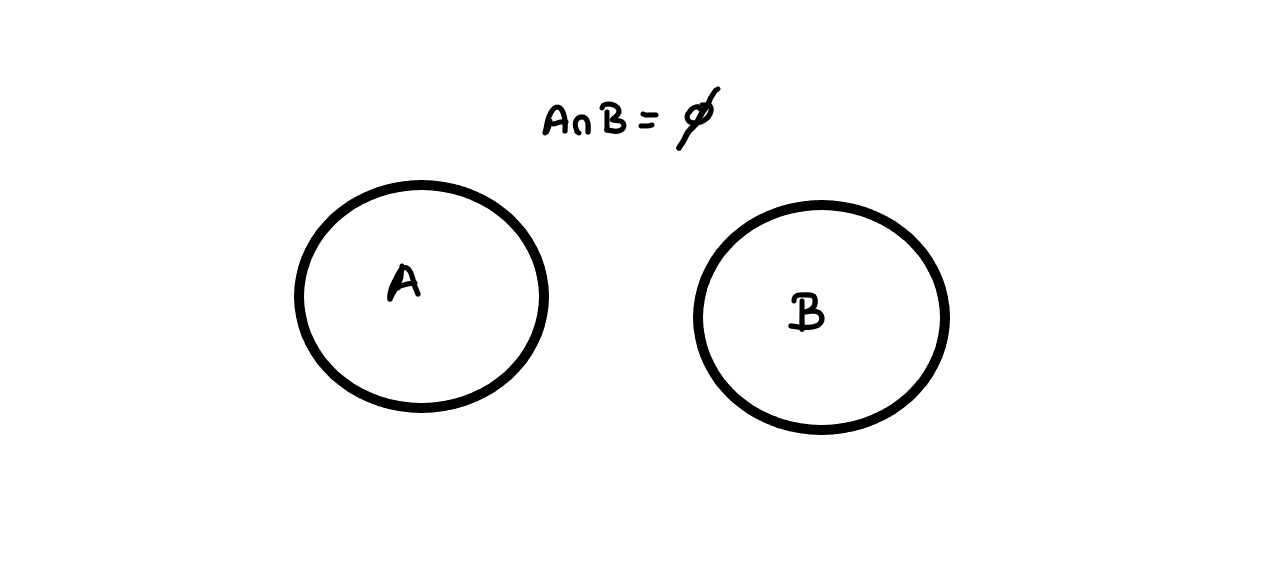
\includegraphics{disjoint.png}
\caption{\label{fig:unnamed-chunk-11}picture showing two disjoint sets}
\end{figure}

\end{definition}

\begin{remark}
Again as with unions, we will more often see this definition applied to sequences of sets using notation like
\[ \bigcap_n A_n.  \]
\end{remark}

\begin{example}
\[ \{1,2,3\} \cap \{ 1,2,4\} = \{1,2\}.\]
\end{example}

\begin{example}
\[\bigcup_{n \in \mathbb{N}} [[n]] = {0}. \]
\end{example}

\begin{lemma}

Given sets \(A, B, C\) the following are true

\begin{itemize}
\item
  \(A \cap \emptyset = \emptyset\),
\item
  \((A \cap B) \cap C = A \cap (B\cap C)\),
\item
  \(A \cap B = B \cap A\),
\item
  \(A \cap B = B\) if and only if \(A \supset B\),
\item
  \(A \cap A = A\).
\end{itemize}

\end{lemma}

\begin{definition}[set difference]

If \(A\) and \(B\) are sets the we define the \emph{set difference} which we write \(A - B\) (or sometimes \(A \setminus B\)) by

\[ A - B = \{ x \,:\, x \in A, x \notin B\}.  \]

\begin{figure}
\centering
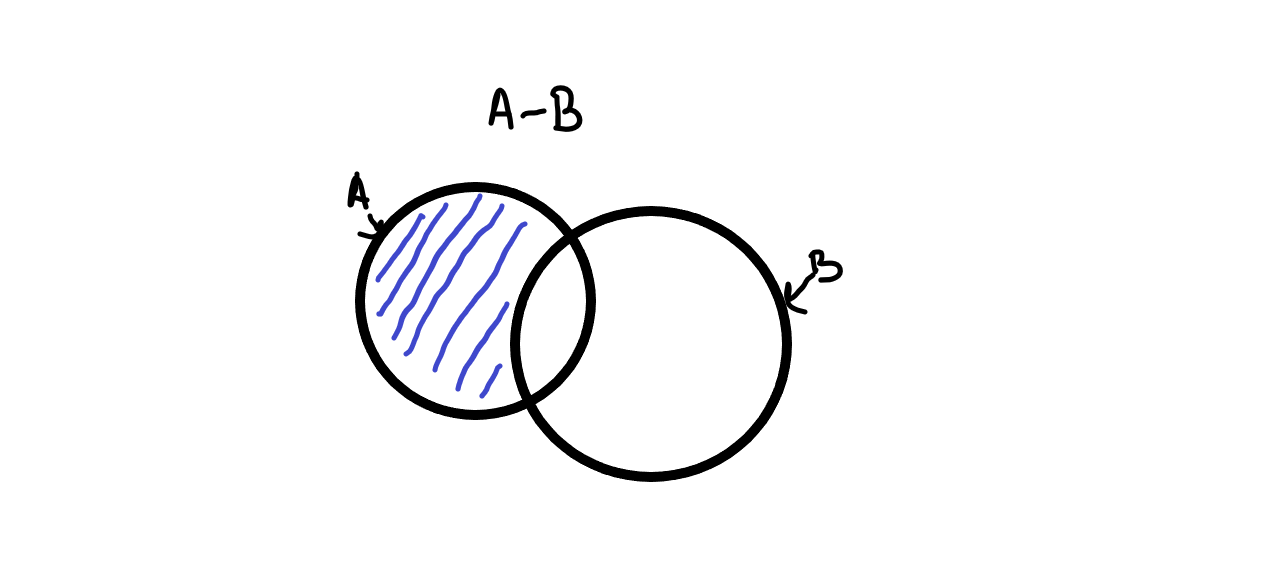
\includegraphics{setminus.png}
\caption{\label{fig:unnamed-chunk-12}picture of setminus with sets represented by overlappying circles}
\end{figure}

\end{definition}

\begin{remark}
WARNING: Unlike union and intersection, set difference is not commutative.
\end{remark}

\begin{example}
\[ \{1,2,3\} - \{1,2,4\} = \{3\}, \quad \{1,2,4\} - \{1,2,3\} = \{4\}.\]
\end{example}

\section{Using set operations together}\label{using-set-operations-together}

There are some rules for how set operations interact with each other. Usually these are easy to remember/prove by drawing pictures or by writing out exactly what each operation means.

\begin{lemma}

Suppose that \(A, B\) and \(C\) are sets then we can distribute intersections and unions with each other in the following way

\begin{itemize}
\tightlist
\item
  \(A \cap (B \cup C) = (A \cap B) \cup (A \cap C)\)
\end{itemize}

\begin{figure}
\centering
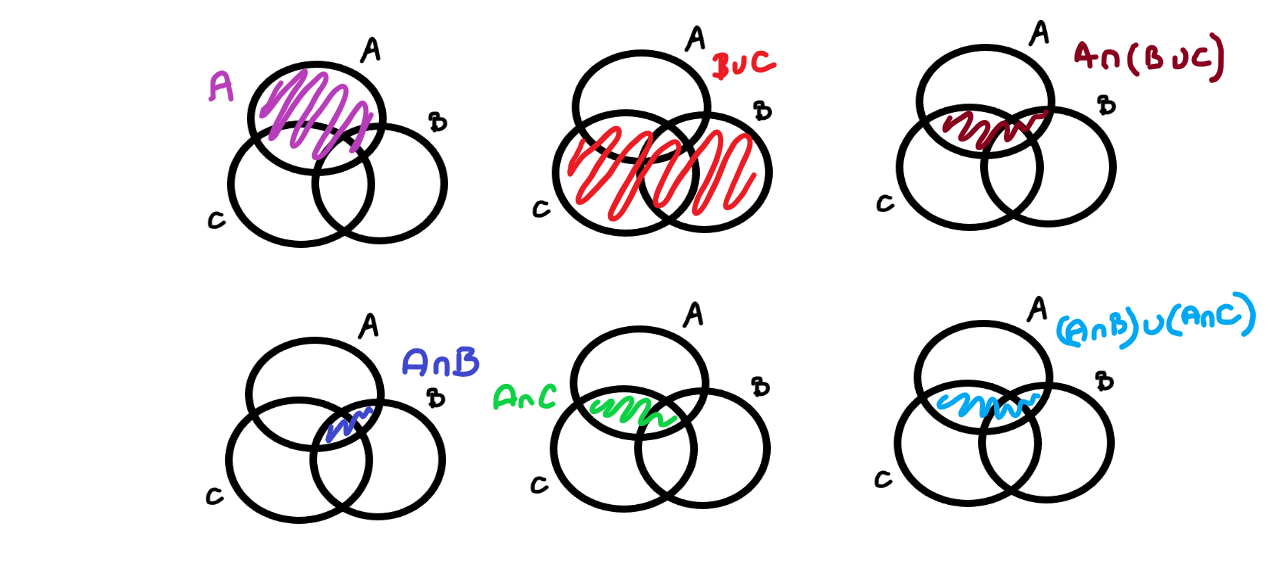
\includegraphics{distributive1.png}
\caption{\label{fig:unnamed-chunk-13}picture of distibutivity of union}
\end{figure}

\begin{itemize}
\tightlist
\item
  \(A\cup (B \cap C) = (A \cup B) \cap (A \cup C)\)
\end{itemize}

\begin{figure}
\centering
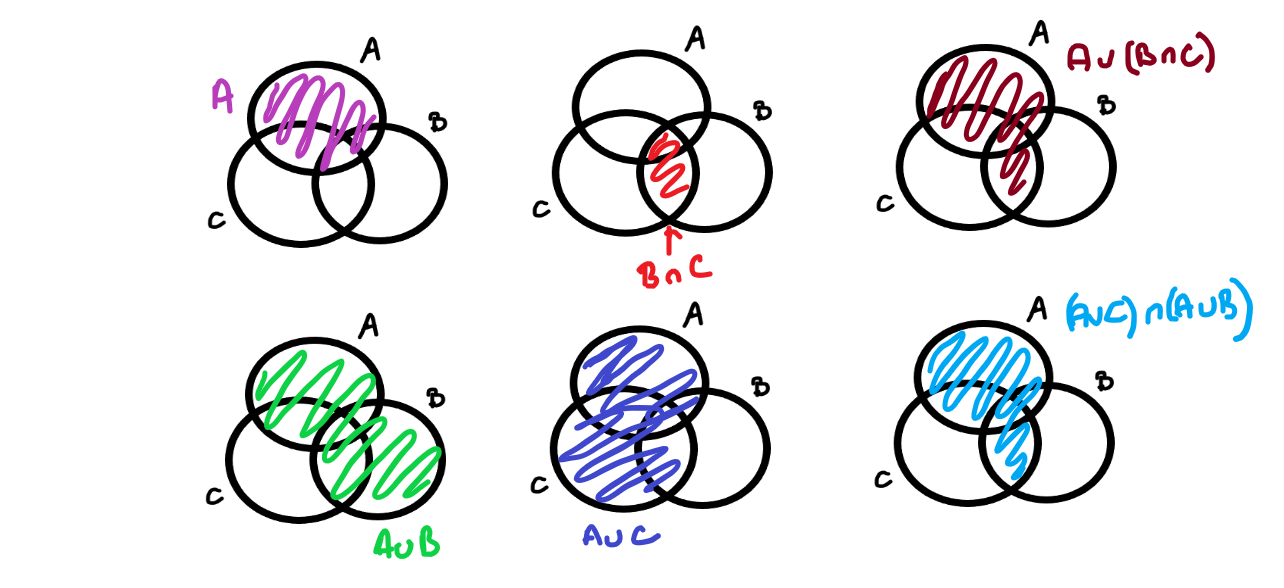
\includegraphics{distributive2.png}
\caption{\label{fig:unnamed-chunk-14}picture of distibutivity of intersection}
\end{figure}

\end{lemma}

\begin{proof}
These results are very straightforward to prove. We remember that that if \(x \in A \Rightarrow x \in B\) and \(x \in B \Rightarrow x \in A\) then \(A = B\).

If \(x \in A \cap (B \cup C)\) then we know \(x \in A\) and \(x \in B\) or \(x \in C\). Therefore \(x \in A\) and \(x \in B\) or \(x \in A\) and \(x \in C\) so \(x \in (A\cap B) \cup (A \cap C)\).

The second result is proved similarly.

As there are only 3 sets involved the pictures probably provide a clearer (and still rigorous) proof for most people. However with four or more sets it becomes impossible to draw sets with all the possible intersections, so we need to be able to use symbols too.
\end{proof}

We also have a similar result involving setminuses.

\begin{lemma}[De Morgan's Laws]

Suppose \(A, B\) and \(C\) are sets then the following are true

\begin{itemize}
\tightlist
\item
  \(A - (B \cup C) = (A-B)\cap(A-C)\),
\end{itemize}

\begin{figure}
\centering
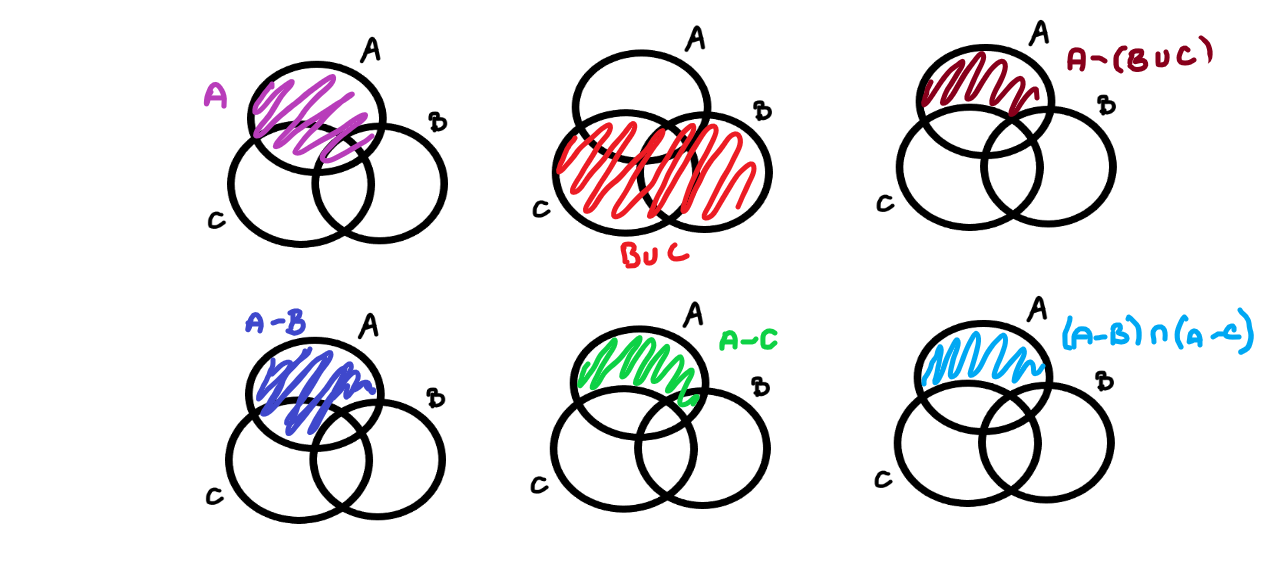
\includegraphics{demorgan1.png}
\caption{\label{fig:unnamed-chunk-15}picture of De Morgan's Laws 1}
\end{figure}

\begin{itemize}
\tightlist
\item
  \(A - (B \cap C) = (A-B)\cup(A-C)\).
\end{itemize}

\begin{figure}
\centering
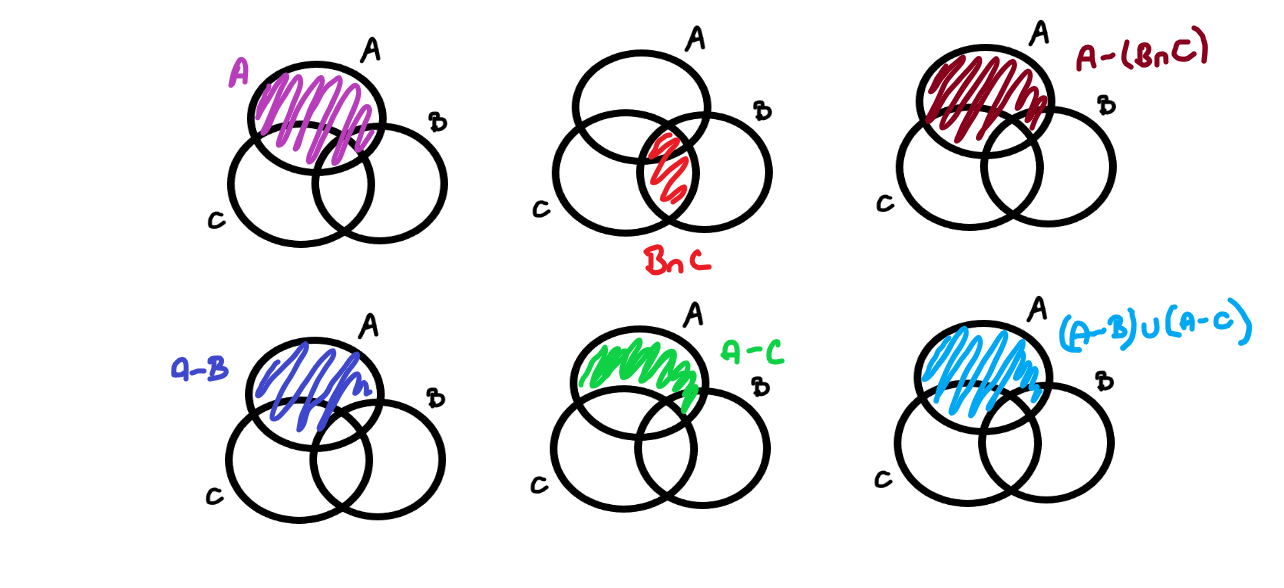
\includegraphics{demorgan2.png}
\caption{\label{fig:unnamed-chunk-16}picture of De Morgan's Laws 2}
\end{figure}

\end{lemma}

All these operations can be understood in terms of indicator functions as well

\begin{lemma}

Given a set \(A\) and subsets \(B, C, D\) we have the following:

\begin{itemize}
\item
  \(1_{B \cap C} = 1_{B}1_{C}\).
\item
  \(1_{B \cup C} = 1_B + 1_C - 1_B 1_C\).
\item
  If \(B \subset C\) then \(1_{C \setminus B} = 1_C - 1_B\).
\end{itemize}

\end{lemma}

\begin{proof}
If you want to you can check these yourself. It is mainly just symbol pushing. A more exciting thing to do is try and prove De Morgan's laws or distributative laws using these facts.
\end{proof}

\section{Operations on functions}\label{operations-on-functions}

\begin{definition}[composition]

Given sets \(A, B\) and \(C\) and functions \(f: A \rightarrow B\) and \(g: B \rightarrow C\) we can define a new function \(f \circ g\) from \(A\) to \(C\) by
\[ f\circ g(x) = g(f(x)).  \]

\begin{figure}
\centering
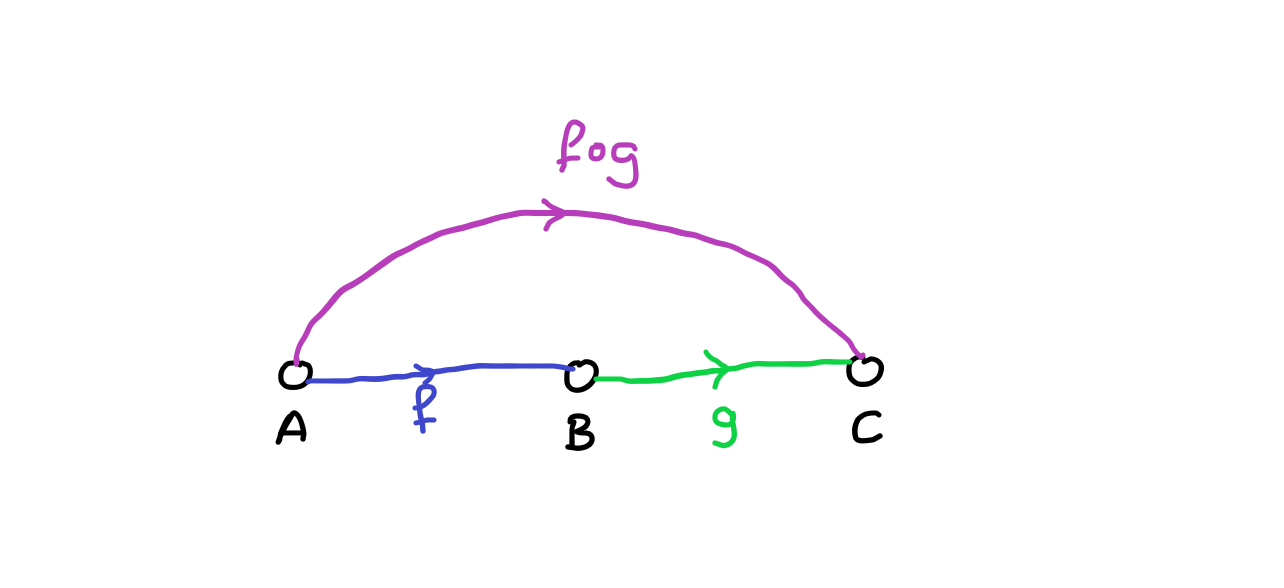
\includegraphics{compositiondiagram.png}
\caption{\label{fig:unnamed-chunk-17}diagram of function composition}
\end{figure}

\end{definition}

\begin{example}

\begin{figure}
\centering
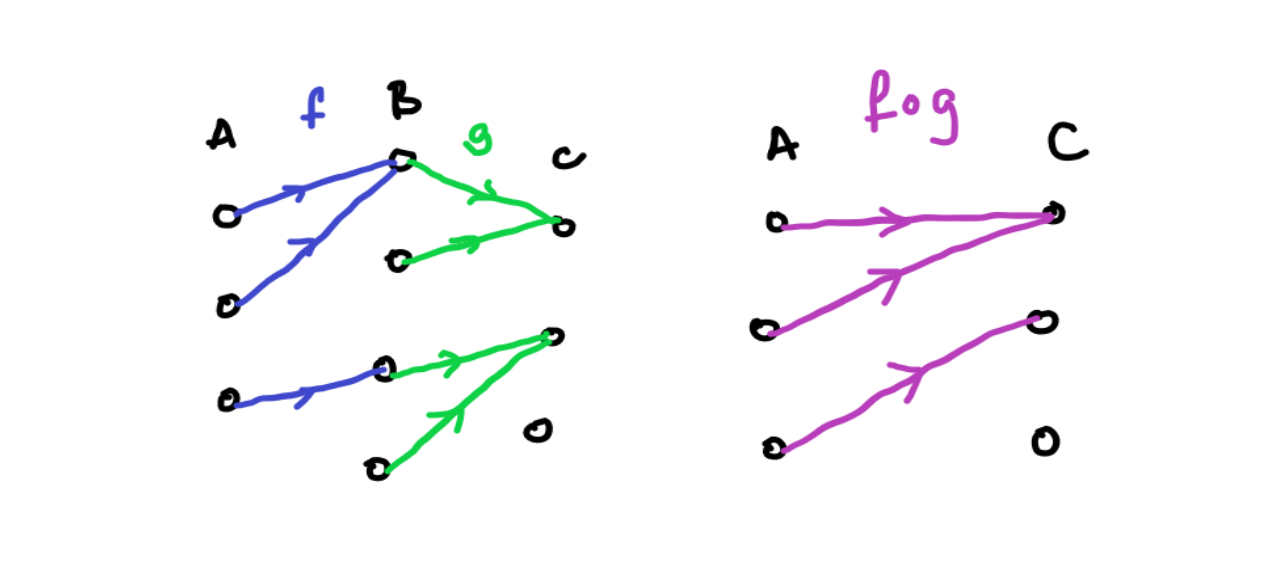
\includegraphics{compositionexample.png}
\caption{\label{fig:unnamed-chunk-18}example of function composition}
\end{figure}

\end{example}

\begin{example}
Another example would be if \(f: \mathbb{R} \rightarrow [0,\infty)\) is defined by \(f(x) = x^2\) and \(g: [0,\infty) \rightarrow [0, \infty)\) is defined by \(g(y) = \sqrt{y}\) then \(f \circ g (x) = |x|\) and is defined from \(\mathbb{R}\) to \([0,\infty)\).
\end{example}

\begin{remark}
An important example of composition is if \(A\) is a set and \(f: A \rightarrow A\) then we can compose \(A\) with itself. We often write \(f\circ f = f^2\) and \(f^n= f\circ f^{n-1}\).
\end{remark}

\begin{lemma}[Associativity of composition]

Composition of functions is associative. That is to say, if \(A,B,C\) and \(D\) are all sets and \(f:A \rightarrow B, g: B \rightarrow C\) and \(h: C \rightarrow D\) are all functions then
\[ f \circ (g \circ h) = (f \circ g) \circ h  \]

\begin{figure}
\centering
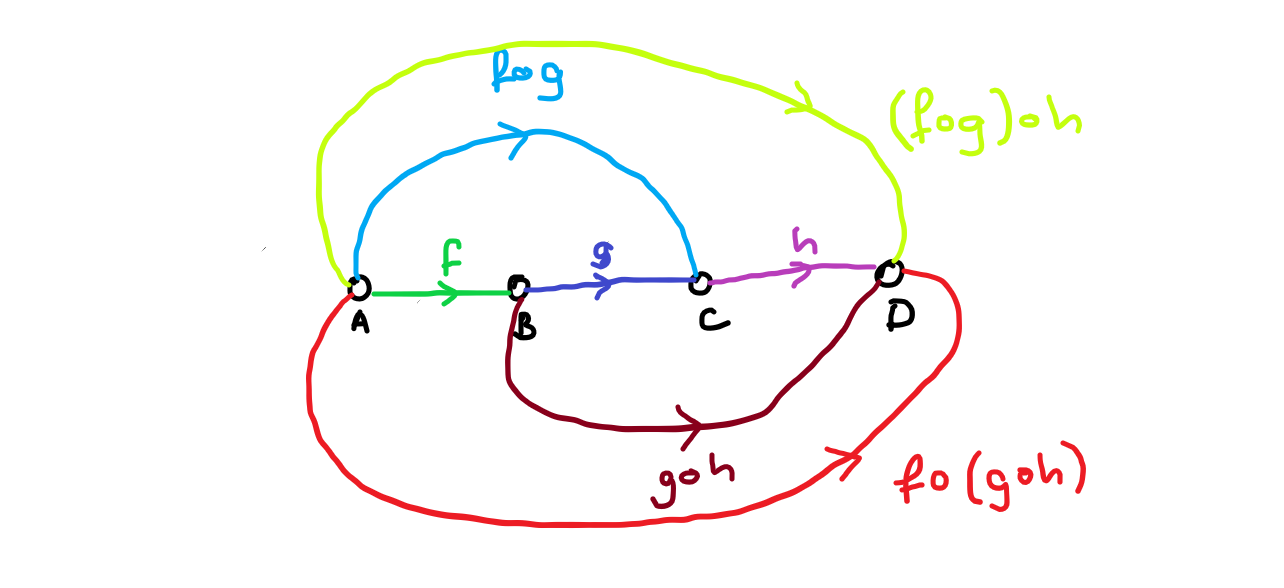
\includegraphics{compassoc.png}
\caption{\label{fig:unnamed-chunk-19}picture of associativity of composition of function}
\end{figure}

\end{lemma}

\begin{proof}
To prove this we can evaluate the functions at a given \(x \in A\).

\[f \circ (g \circ h)(x) = (g \circ h)(f(x)) = h(g(f(x))).\]

\[(f\circ g) \circ h(x) = h (f\circ g(x)) = h(g(f(x))).\]
\end{proof}

We can relate composition of functions to injectivity and surjectivity

\begin{lemma}

Suppose that \(A, B\) and \(C\) are sets and \(f: A \rightarrow B\) and \(g: B \rightarrow C\) are functions then

\begin{itemize}
\item
  If both \(f\) and \(g\) are injective then so is \(f \circ g\),
\item
  If both \(f\) and \(g\) are surjective then so is \(f \circ g\).
\end{itemize}

\end{lemma}

\begin{proof}
If both \(f\) and \(g\) are injective then given \(z \in C\) there is at most one \(y \in B\) with \(g(y)=z\) then for this \(y\) there is at most one \(x \in A\) with \(f(x) = y\) therefore there is at most one \(x \in A\) with \(f\circ g(x) = z\).

If both \(f\) and \(g\) are surjective then given \(z \in C\) there is at least one \(y \in B\) with \(g(y) = z\) and for this \(y\) there is at least one \(x \in A\) with \(f(x) = y\) therefore there is at least one \(x \in A\) with \(f \circ g (x) = z\).
\end{proof}

This next set of results is about what it means to be the \emph{inverse of a function}. This can be a subtle and quite complicated issue.

\begin{example}
As we just saw above if \(f: \mathbb{R} \rightarrow [0,\infty)\) is defined by \(f(x) = x^2\) and \(g: [0,\infty) \rightarrow [0, \infty)\) is defined by \(g(y) = \sqrt{y}\) then \(f \circ g (x) = |x|\). So even though we think of square root and squaring as inverses of each other in this case \(f \circ g\) is not equal to the identity function.

On the other hand if \(f : [0, \infty) \rightarrow [0, \infty)\) defined by \(f(x)=x^2\) and \(g: [0,\infty) \rightarrow [0,\infty)\) is defined by \(g(y) = \sqrt(y)\) then \(f \circ g(x) = x\) so if we change the domain of \(f\) we can think for these functions as inverse to each other.

We also have that if \(f: \mathbb{R} \rightarrow [0,\infty)\) defined by \(f(x) = x^2\) and \(g: [0, \infty) \rightarrow [0,\infty)\) defined by \(g(y) = \sqrt(y)\) (as in the first part of the example) then \(g\circ f)(y) = y\). we can think of these as inverse to eachother in one order but not in the other order.
\end{example}

\begin{definition}[left and right inverses]

Let \(A\) and \(B\) be sets and let \(f: A \rightarrow B\) and \(g: B \rightarrow A\).

\begin{itemize}
\item
  We call \(g\) a \emph{left inverse} of \(f\) if \(g\circ f = Id_B\),
\item
  We call \(g\) a \emph{right inverse} of \(f\) if \(f\circ g = Id_A\).
\item
  We call \(g\) an \emph{inverse} of \(f\) if it is both a left inverse and a right inverse. If an inverse exists we often write \(g = f^{-1}\).
\end{itemize}

\end{definition}

\begin{figure}
\centering
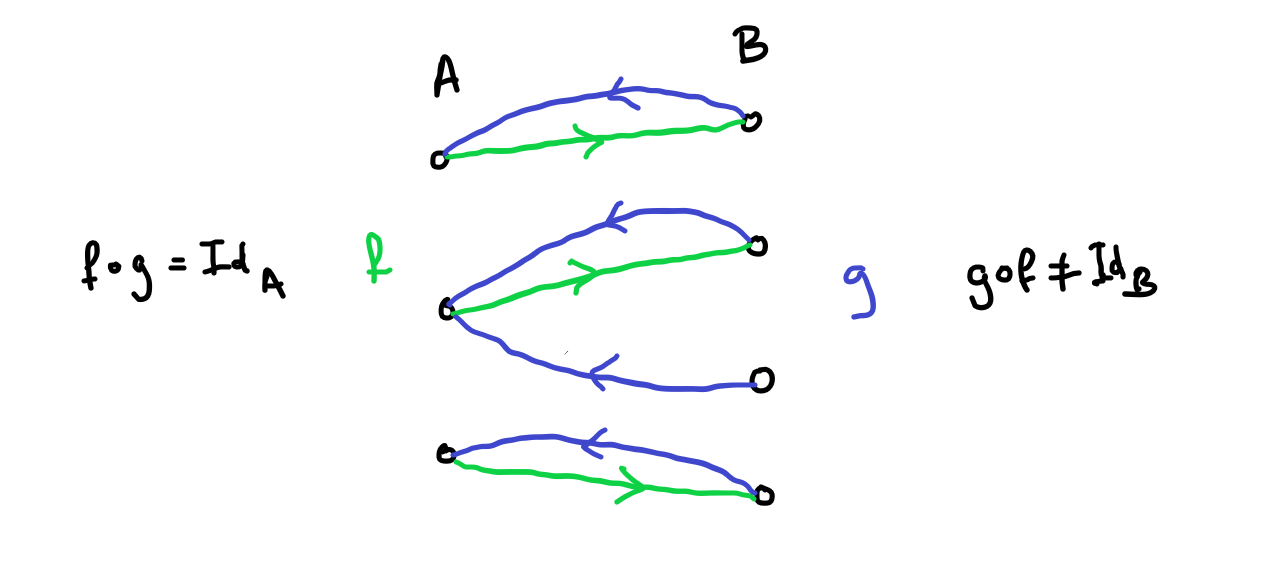
\includegraphics{leftrightinverse.png}
\caption{\label{fig:unnamed-chunk-20}example of a function with a right inverse but no left inverse}
\end{figure}

\begin{lemma}

Given two sets \(A\) and \(B\) and a function \(f: A \rightarrow B\), we have the following equivalences

\begin{enumerate}
\def\labelenumi{\arabic{enumi}.}
\item
  \(f\) is injective if and only if \(f\) has a left inverse,
\item
  \(f\) is surjective if and only if \(f\) has a right inverse,
\item
  \(f\) is bijective if an only if \(f\) has an inverse.
\end{enumerate}

\end{lemma}

\begin{proof}
Let us begin with point 1. in the direction \emph{injective} \(\Rightarrow\) \emph{left inverse}. Injectivity means that for every \(y \in B\) there is at most one \(x \in A\) with \(f(x) = y\). So we can define a left inverse as follows: if there exists an \(x \in A\) with \(f(x)=y\) then set \(g(y) =x\). If there exists no \(x \in A\) with \(f(x)=y\) then choose an arbitrary element \(x_0 \in A\) and set \(g(y) = x_0\). This ensures that for every \(x \in A\) we have \(g(f(x))= x\).

Now point 1 in the direction \emph{left inverse} \(\Rightarrow\) \emph{injective}. So there exists \(g\) with \(g(f(x))=x\) for all \(x \in A\). Suppose \(f\) isn't injective then there exists \(y_0 \in B\) and \(x_1 \neq x_2 \in A\) such that \(f(x_1) = f(x_2) = y_0\). Then we have that \(g(y_0) = g(f(x_1))= x_1 = g(f(x_2))=x_2\) which is a contradiction. Therefore \(f\) must be injective.

Now point 2 in the direction \emph{surjective} \(\Rightarrow\) \emph{right inverse}. For every \(y \in B\) there exists at least one \(x\) such that \(f(x)=y\) by surjectivity. So define a function \(g\) by choosing \(g(y)\) to be equal to one of the \(x \in A\) with \(f(x) = y\). This means that \(f(g(y))= y\) so \(g\) is a right inverse to \(f\).

Now point 2 in the direction \emph{right inverse} \(\Rightarrow\) \emph{surjective}. So we have a function \(g\) such that \(f(g(y))=y\). So for every \(y \in B\) there exist one element in A, namely \(g(y)\), such that \(f(g(y))=y\) so \(f\) is surjective.

Now for point 3 it looks at first like we can just apply the previous results. We can in one direction. If \(f\) has an inverse then it has both a left inverse and a right inverse so by points 1 and 2 \(f\) must be both injective and surjective so it is bijective.

Now if we want to show bijectivity of \(f\) implies we must have an inverse we not that if \(f\) is bijective then for every \(y\in B\) there exists exactly one \(x \in A\) such that \(f(x) = y\) so we can define \(g(y)\) to be this unique \(x\) and this ensures that \(g(f(x))= x\) and \(f(g(y))= y\).
\end{proof}

\begin{definition}[pigeon hole principle]
Suppose \(A\) and \(B\) are finite sets with \(|A| > |B|\) and \(f: A \rightarrow B\) is a function then there exists some \(b \in B\) for which there are at least two elements \(a_1,a_2\) of \(A\) for which \(f(a_1)=f(a_2)=b\).

The name for this fact comes from the idea that if you have a dovecote with \(n\) holes and you have more than \(n+1\) pigeons then however you arrange the pigeons at least one hole must contain more than one pigeon.
\end{definition}

\begin{lemma}

Suppose that \(A,B\) are sets and \(B\) is finite.

\begin{itemize}
\item
  If there exists an injection \(f: A \rightarrow B\) then \(A\) is finite.
\item
  If there exists a surjections \(g: B \rightarrow A\) then \(A\) is finite.
\end{itemize}

\end{lemma}

\begin{proof}
If \(B\) is finite then there is a bijection between \(B\) and some \([[n]]\) and so composing \(f\) and this bijection gives an injection form \(A\) to some subset of \([[n]]\). Let us call this injection \(j\). Now let us create a bijection from \(A\) to some \([[m]]\) as follows. The image of \(j\) is \(\{j_0, \dots, j_m\}\) so let us map \(j^{-1}(j_k)\) to \(k\) for \(k=0,\dots, m\). This shows that \(A\) is finite.

Now considering the second point. We can choose a right inverse to \(g\) which we call \(h\). This will be an injection since \(g\) is a function so the first point proves that \(A\) is finite also in this case.
\end{proof}

Lastly in this section we have a deeper theorem whose proof is more complicated that those we have encountered before.

\begin{theorem}[Cantor-Schoeder-Bernstein]
Let \(A, B\) be sets and let \(f: A \rightarrow B\) be an injection and \(g: B \rightarrow A\) be an injection. Then there exists a bijection \(h\) between \(A\) and \(B\).
\end{theorem}

\begin{proof}[NONEXAMINABLE]
Let us call \(C = f(A) \subset B\) and \(D = g(B) \subset A\). Since \(f\) and \(g\) are injective we can define \(f^{-1}:C \rightarrow A\) and \(g^{-1}: D \rightarrow B\).

So we end up with two bijective functions going from parts of \(A\) to parts of \(B\) namely \(f: A \rightarrow D\) and \(g^{-1}: C \rightarrow B\)

\begin{figure}
\centering
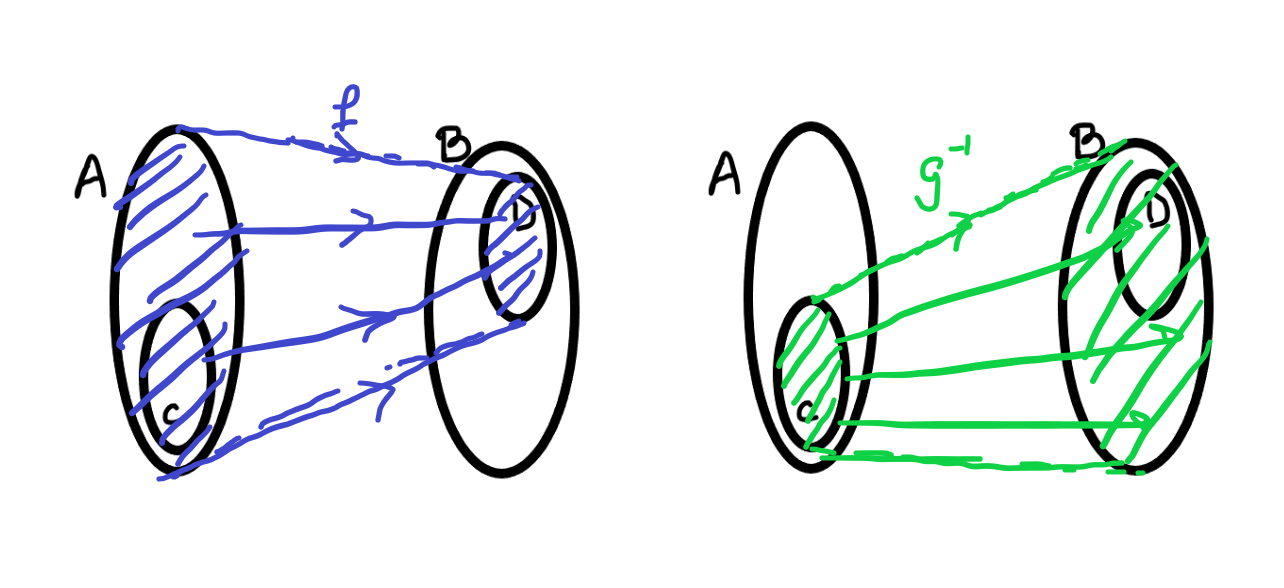
\includegraphics{CBS1.png}
\caption{\label{fig:unnamed-chunk-21}Our two functions going from A to B}
\end{figure}

Now we want to create \(h\) from both \(f\) and \(g^{-1}\). To do this we want to split \(A\) into two sets \(A_1\) where we use \(f\) to get to points in \(B\) and \(A_2\) where we use \(g^{-1}\) to get to points in \(B\).

\begin{figure}
\centering
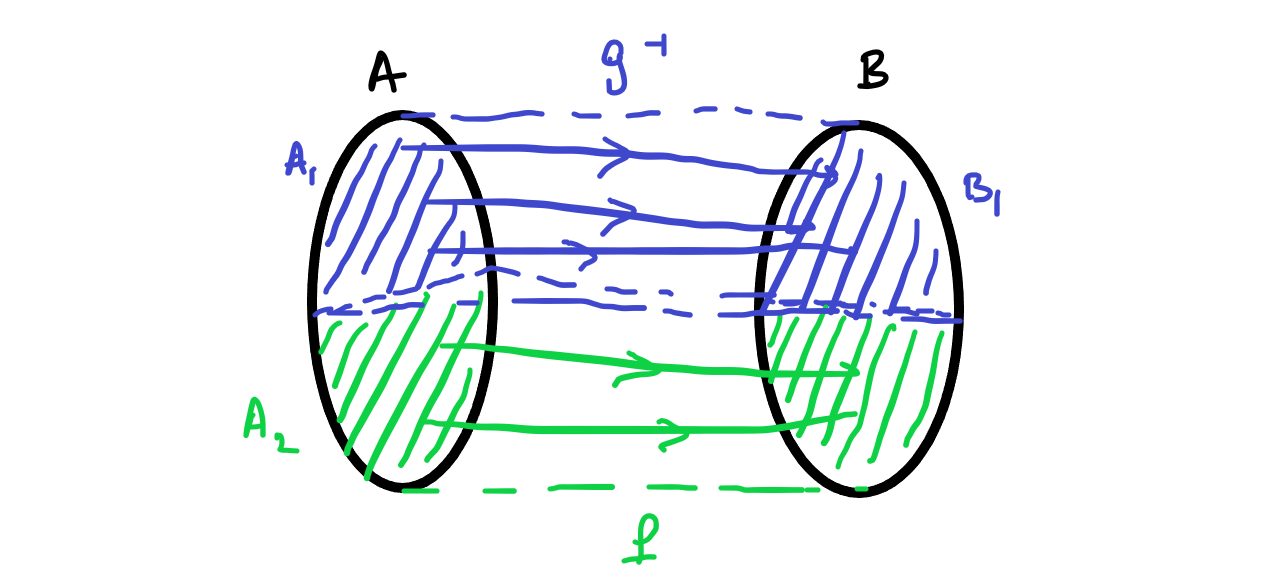
\includegraphics{CBS2.png}
\caption{\label{fig:unnamed-chunk-22}A picture of how we want to split up A}
\end{figure}

Our challenge is to find suitable sets \(A_1\) and \(A_2\). We can see that \(A_2 \subset C\) since \(g^{-1}\) must be defined on \(A_2\). We can also see that in some situations \(A_2\) could be the whole of \(C\) because doing this we could hit some elements of \(D\) twice and break the injectivity.

Let us write \(i = f\circ g\). This function is injective on \(A\) and it's range is \(C\). We can similarly define \(j = g \circ f\) which will also be injective on \(B\) and whose range is \(D\).

Now let us create some sequences of sets \(C_0 = A, C_1 = i(A), C_2=i(C_1), \dots, C_n = i(C_{n-1}), \dots\) and \(D_0 = B, D_1= j(B), \dots, D_n = j(D_{n-1}), \dots\). Then let us define \(C_\infty = \bigcap_n C_n\) and \(D_\infty = \bigcap_n D_n\). So \(C_\infty\) are points which will keep being in the range of \(i^n\) for any \(n\) and \(D_\infty\) similarly.

We make the following claim:
\begin{align}
g(y) \in C_\infty &\Leftrightarrow y \in D_\infty, \\
f(x) \in D_\infty &\Leftrightarrow x \in C_\infty.
\end{align}

Let us call
\[ A_1 = \{ x \in A \,:\, x \notin C_\infty, \mbox{for the least} \,n \, \mbox{s.t.}\, x \notin C_n, i^{-n+1}(x) \notin C\} \]
and
\[ A_0 = \{ x \in A \,:\, x \notin C_\infty, \mbox{for the least} \, n \, \mbox{s.t.}\, x \notin C_n, i^{-n+1}(x) \in C, g^{-1}(i^{-n+1}(x)) \notin D \}.\] Then \(A_1\) and \(A_2\) are disjoint.

Similarly,

\[ B_1 = \{y \in B\,:\, y \notin B_\infty, \mbox{for the least}\, n \, \mbox{s.t.}\, y \notin D_n, j^{-n+1}(y) \notin D\}\]
and
\[ B_0 = \{y \in B\,:\, y \notin B_\infty, \mbox{for the least}\, n \, \mbox{s.t.}\, y \notin D_n, j^{-n+1}(y) \in D, f^{-1}(j^{-n+1}(y)) \notin C\}.\] The sets are also disjoint.

Now we have our second claim:

\begin{itemize}
\item
  \(x \in A_1\) if and only if \(f(x) \in B_0\)
\item
  \(x \in A_0\) if and only if \(g^{-1}(x) \in B_1\)
\end{itemize}

This second claim shows that

\begin{itemize}
\item
  \(f|_{A_1} : A_1 \rightarrow B_0\) is a bijection and
\item
  \(g^{-1}|_{A_0} : A_0 \rightarrow B_1\) is a bijection.
\end{itemize}

\begin{figure}
\centering
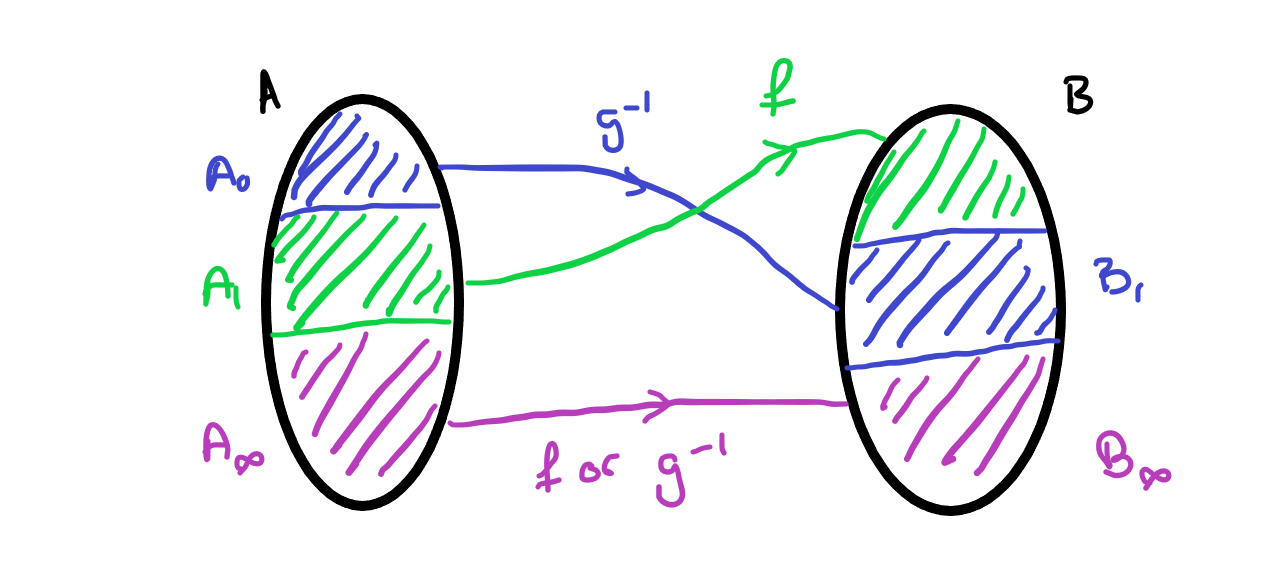
\includegraphics{CBS3.png}
\caption{\label{fig:unnamed-chunk-23}A picture of the bijections we've constructed}
\end{figure}

Now we have deconstructed into different bijections we can define \(h\) by saying
\[ h(x) = \left\{ \begin{array}{cr} f(x) & x \in A_1 \cup A_\infty\\ g^{-1}(x) & x \in A_0 \end{array} \right.  \]
\end{proof}

\chapter{Relations}\label{relations}

Before we define them formally let us look at some examples.

For a generic relationship \(R\) we write \(x\) and \(y\) are related under \(R\) by \(x R y\). Here the ordering matters as you can see in the example.

\begin{example}
We can relate two real numbers \(x\) and \(y\) with the relationship \emph{is less than}. So we can write \(xR y\) if \(x \leq y\).
\end{example}

\begin{example}
Is equal to is also a relation. This can be more complicated that just trivially equating elements of the same set. For example we might want to write a relation between \(\mathbb{N}\) and \(\mathbb{R}\) by equating integers with their counterpart in the natural numbers.
\end{example}

\begin{remark}
Something that isn't a relation but might seem similar is a \emph{property}. So for example the statement \(3\) is a prime number is just talking about a property that may or may not hold for the integers. We can come up with a relation to the set \(\{1\}\) by saying \(n R 1\) if and only if \(n\) is prime.
\end{remark}

The formal definition of a relation is as follows

\begin{definition}[relation]
A relation consists of three parts

\begin{itemize}
\item
  A set \(X\) called the \emph{domain},
\item
  A set \(Y\) called the \emph{co-domain}
\item
  A subset of \(X \times Y\) often given the name \(R\).
\end{itemize}

Using the notation from before we write \(x R y\) iff \((x,y)\) is in the subset of \(X \times Y\) defining the relation.
\end{definition}

We can represent the relation \emph{is less than} with a picture as we saw in week 1.

\begin{figure}
\centering
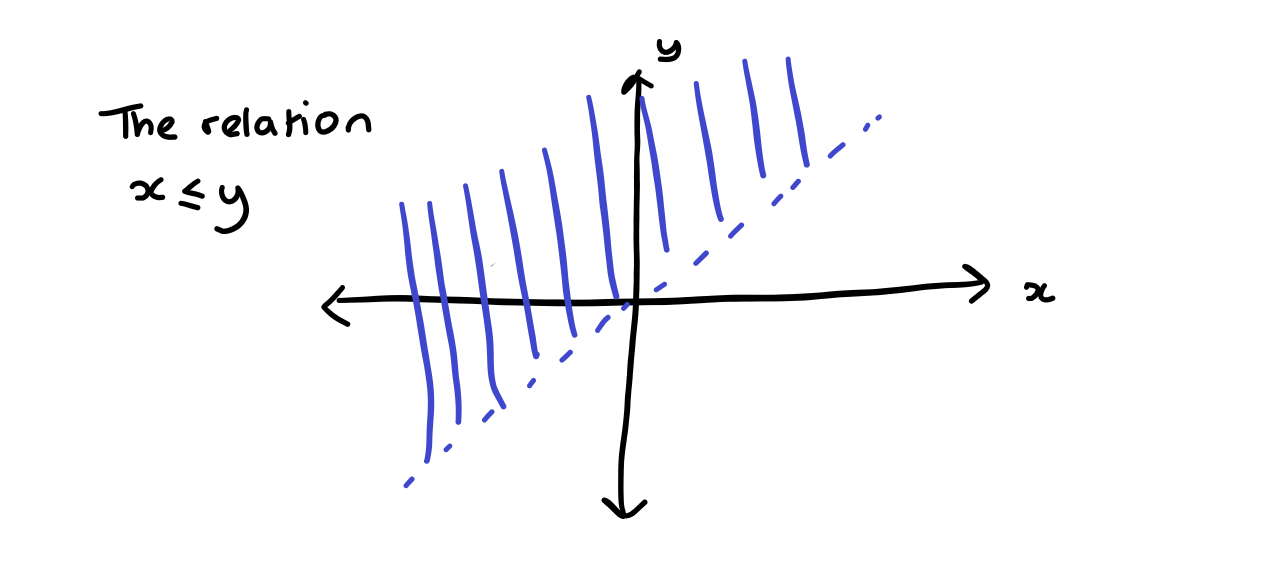
\includegraphics{less than.png}
\caption{\label{fig:unnamed-chunk-24}A picture of the relation less than}
\end{figure}

\section{Equivalence relations, Equivalence classes and Quotients}\label{equivalence-relations-equivalence-classes-and-quotients}

In this section we look at some particular properties a relation can have when it relates elements of the same sets. That is to say, we are interested in a set \(X\) and a relation \(R\) on \(X\) defined by a subset of \(X^2\).

\begin{definition}[reflexivity]
We call a relation, \(R\), on \(X\) \emph{reflexive} if \(x R x\).
\end{definition}

\begin{example}
The relation defined by \(<\) is \emph{not} reflexive; the relation defined by \(\leq\) \emph{is} reflexive.
\end{example}

\begin{definition}[transitivity]
We call a relation \(R\) on \(X\) \emph{transitive} if \(x R y\) and \(y R z\) implies that \(x R z\).
\end{definition}

\begin{example}
Both the relations given above \(<,\leq\) are transitive but a relation like \emph{is the square of} is not.
\end{example}

\begin{definition}[symmetric]
A relation \(R\) on \(X\) is \emph{symmetric} if \(x R y\) implies that \(y R x\).
\end{definition}

\begin{example}
The relation on \(\mathbb{R}\) given by \(xR y\) if an only if \(|x-y|=1\) is symmetric.

The relation on \(\mathbb{R}\) given by \(x R y\) if and only if \(x-y=1\) is not symmetric.
\end{example}

\begin{definition}[equivalence relations]
A relation on \(X\) is called an \emph{equivalence relation} if it is reflexive, symmetric and transitive. We often denote equivalence relations with \(\sim\) rather than \(R\).
\end{definition}

\begin{remark}
Equivalence relations are a very important object in mathematics. We will see more about splitting up sets using equivalence relations soon. Equivalence relations are supposed to represent the properties of equality.
\end{remark}

\begin{example}

\begin{itemize}
\item
  The relation defined by \(x \sim y\) if and only if \(x-y \in \mathbb{Q}\) is and equivalence relation.
\item
  The relation defined by \(x \sim y\) if and only if \(x=y\) is an equivalence relation.
\end{itemize}

\end{example}

We can use equivalence relations to divide sets into chunks. In order to talk about this let us first give a proper definition of what it would mean to define a set into chunks.

\begin{definition}[Partitions]

Given a set \(X\) a partition of \(X\) is a subset \(\mathbb{P}\) or \(\mathcal{P}(X)\) (so a set of subsets of \(X\)) satisfying the following:

\begin{itemize}
\item
  If \(P, Q\) in \(\mathbb{P}\) and \(P \neq Q\) then \(P \cap Q = \emptyset\), i.e.~any two sets in \(\mathbb{P}\) are disjoint,
\item
  \(\bigcup_{P \in \mathbb{P}}P = X\), i.e.~for every \(x \in X\) there is a \(P \in \mathbb{P}\) such that \(x \in P\),
\item
  Every \(P \in \mathbb{P}\) is non-empty.
\end{itemize}

\end{definition}

\begin{figure}
\centering
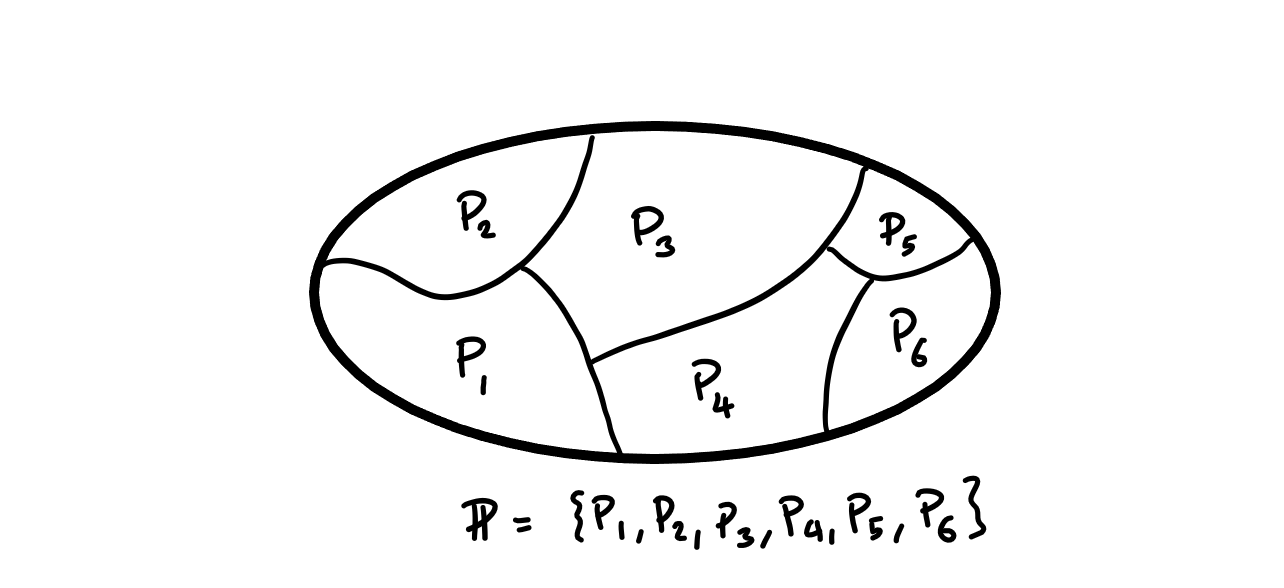
\includegraphics{partition.png}
\caption{\label{fig:unnamed-chunk-25}A picture of a partition}
\end{figure}

\begin{example}
For any \(X\) we can define the partition into the set of singletons, \(\mathbb{P}= \bigcup_{x \in X}\{\{x\}\}\).

We can also define a trivial partition \(\mathbb{P} = X\).
\end{example}

We can use equivalence relations to form partitions. First let us talk about each of the chunks separately.

\begin{definition}[equivalence class]
Given a set \(X\) and an equivalence relation \(\sim\) and an element \(x \in X\) we define the equivalence class of \(x\) by
\[ E_x = \{ y \in X \,:\, x \sim y\}.\]
Another common notation for this is \([x]\) or \([x]_\sim\).
\end{definition}

\begin{lemma}
Given a set \(X\) and an equivalence relation \(\sim\) then the equivalence classes under \(\sim\) form a partition of \(X\).

Equally, given a set \(X\) and a partition \(\mathbb{P}\) of \(x\) the relation defined by \(x \sim y\) if \(x\) and \(y\) are both in the same \(P\).
\end{lemma}

\begin{proof}

\begin{itemize}
\item
  For every \(x \in X\) we know that \(x \in E_x\) so the union of all equivalence classes is all of \(X\).
\item
  If \(E, F\) are two equivalence classes then if there exists \(x \in E \cap F\) then \(y \sim x\) for every \(y \in E\) and \(z \sim x\) for every \(z \in F\). So by transitivity of \(\sim\) we have \(y \sim z\) for every \(y \in E, z \in F\) therefore we must have \(E=F\).
\item
  Every equivalence class is not empty as \(x \sim x\) so \(x \in E_x\).
\end{itemize}

This proves that the equivalence classes form a partition of the set.

Now considering \(\sim\) defined in the lemma.

\begin{itemize}
\item
  It is reflexive since \(x \in P\) so \(x \sim x\).
\item
  It is transitive since if \(x \sim y\) and \(y \sim z\) then \(x \in P\) implies \(y \in P\) which in turn implies \(z \in P\) so \(x \sim z\).
\item
  It is symmetric since if \(x \sim y\) then for some \(P\),\(x, y \in P\) so \(y \sim x\).
\end{itemize}

\end{proof}

\begin{example}
If we consider the equivalence relation on \(\mathbb{Z}\) given by \(x \sim y\) when \(|x-y|\) is divisible by \(2\). Then under this relation we have two equivalence classes. The even integers and the odd integers.
\end{example}

\subsection{Quotients}\label{quotients}

While it probably won't be obvious in this course quotients are one of the most important concepts in mathematics. Quotienting by an equivalence relation is the act of considering two objects to be \emph{the same} if they lie in the same equivalence class. In further areas of mathematics you will be considering sets with structures on them (e.g.~groups in algebra) and when you quotient by things you will want to do so in such a way that you can preserve that structure. At the moment we are only interested in the structure of being a set. That is crucially the axiom of extension that a set is defined by its elements.

\begin{definition}[quotient]
Given a set \(X\) and an equivalence relation \(\sim\) then we define the quotient
\[ X/\sim = \{\mbox{the set of equivalence classes under \(\sim\)}\}= \{ E_x \,:\, x \in X\}.\]
\end{definition}

\begin{example}
If we consider the set \(\mathbb{R}\) and the equivalence relation \(x \sim y\) when \(x-y \in \mathbb{Z}\). Then for any \(x\) the set \(E_x\) is the set of all real numbers who have the same decimal expansion after the decimal point we often call this set \(\mathbb{T}\) and think about it as wrapping the real numbers repeatedly around the set \([0,1)\).
\end{example}

\begin{example}
Quotienting by equivalence relations is one example of using mathematical abstraction. It is something you will already have been doing very frequently. A good example from school mathematics is congruent triangles. We call triangles similar if they have the same angles and side length. Regarding two triangles as \emph{the same} if they are congruent is an example of quotienting by an equivalence relation.
\end{example}

\section{Integers via quotients}\label{integers-via-quotients}

Quotients are a key way of constructing new things from old. A good example is constructing \(\mathbb{Z}\) starting from \(\mathbb{N}\).

We work from the starting point that we have defined \(\mathbb{N}\) and addition and multiplication on \(\mathbb{N}\) already.

\begin{definition}[Integers]

In this setting we want to think about integers as the possible differences between two natural numbers. So, for example, we want to define \(-1 = 2-3\), or anything representing taking one step to the left on the numberline. So we want to construct the integers from ordered pairs of natural numbers \(\mathbb{N}^2\). We can make a direct equivalence between \(\mathbb{N}^2\) and \(\mathbb{Z}\) because there are many possible pairs of natural numbers whose difference will be equal to the same integer e.g.~\(-1=2-3=4-5\). So we need to put an equivalence relation on \(\mathbb{N}^2\) so we have
\[ (p, q) \sim (s,t) \, \mbox{when} \, p+t=s+q.  \]
Then we can identify \(\mathbb{Z}\) with \(\mathbb{N}^2/\sim\).

Now we want to further define the arithmetic operations on \(\mathbb{Z}\) we do this as follows.

\begin{itemize}
\item
  We define a function called \emph{negation} by \(-:\mathbb{Z} \rightarrow \mathbb{Z}\) by \(-E_{(p,q)} = E_{(q,p)}\).
\item
  We define \emph{addition} as a function \(+: \mathbb{Z}^2 \rightarrow \mathbb{Z}\) by \(E_{(p,q)} + E_{(s,t)} = E_{(p+s, q+t)}\).
\item
  We define \emph{multiplication} as a function \(\times : \mathbb{Z}^2 \rightarrow \mathbb{Z}\) by \(E_{(p,q)} \times E_{(s,t)} = E_{(pr+qs, ps+qr)}\).
\end{itemize}

\end{definition}

These definitions show a very common subtlety. We have a function whose domain is a quotient and we specify the function by looking at one element of an equivalence class and specifying the function on that. What we want to do is:

\begin{definition}[well defined function]
Suppose we have a set \(X\), and equivalence relation on \(X\) given by \(\sim\) and we wish to define a function from \(f: X/\sim \rightarrow Y\) by \(f(E_x) = \tilde{f}(x)\) for some other function \(\tilde{f}\). We call \(f\) a \emph{well-defined function} if \(f(x) = f(x')\) whenever \(x \sim x'\).
\end{definition}

You can now ``have fun'' by checking that negation, addition and multiplication as defined above are well defined.

\section{Order relations}\label{order-relations}

\begin{definition}[antisymmetry]
We call a relation \(R\) on \(X\) \emph{antisymmetric} if \(x R y\) and \(y R x\) implies that \(x=y\).
\end{definition}

\begin{example}
The relation above \(x R y\) if and only if \(x-y=1\) is antisymmetric.
\end{example}

\begin{definition}[partial orders]
Partial orders are another special kind of relation on a set. A relation \(R\) on a set \(X\) is a partial order if it is antisymmetric, transitive and reflexive.
\end{definition}

\begin{example}
The most classical example of a partial order is the normal sense of order given by \(\leq\) on some set of numbers \(\mathbb{R}, \mathbb{Q}, \mathbb{Z}, \dots\).

Another example of a partial order is if \(A\) is a set and \(X = \mathcal{P}(A)\) then we can put a partial order on \(X\) with \(B R C\) iff \(B \subset C\). You can check this satisfies all the conditions.
\end{example}

\begin{remark}
These two examples show two key types of partial order. In the first for any two numbers \(x,y\) either \(x \leq y\) or \(y \leq x\). However for any two subsets \(B, C\) it is not the case that either \(B \subset C\) or \(C \subset B\).
\end{remark}

\begin{definition}[total order]
A total ordering on a set \(x\) is a partial order where for every \(x,y\) either \(xRy\) or \(yRx\).
\end{definition}

\section{Modular arithmetic}\label{modular-arithmetic}

We now return to \(\mathbb{N}\) we can define a relation called \emph{is a divisor of} which we write \(n|m\) as \(n\) is a divisor of \(m\).

\begin{definition}[divisor]
Given two natural numbers \(n\) and \(m\) we say \(n\) is a divisor of \(m\) (or \(n|m\)) if there exists \(k \in \mathbb{N}\) such that \(m=n\times k\).
\end{definition}

\begin{remark}
This relation gives us a new example of a partial order on \(\mathbb{N}\). You can check this!
\end{remark}

\begin{definition}[prime number]
While we define divisor it is worth defining a prime number. We call \(p \in \mathbb{N}\) a \emph{prime number} if the only divisors of \(p\) are \(1, p\).
\end{definition}

\begin{definition}[congruence modulo n]
Given an number \(n \in \mathbb{N}-\{0\}\) we can define an equivalence relation on \(\mathbb{Z}\) called congruence modulo n (written \(\equiv\) mod \(n\)) by
\[ p \equiv   q \, (\mbox{mod} \, n) \quad \mbox{when} \quad n\Big| |p-q|.   \]
\end{definition}

\begin{remark}
You can check that congruence modulo \(n\) is an equivalence relation.

We write \([a]_n\) for the equivalence class of an integer \(a\) under congruence modulo \(n\).

We have a slightly different notation for the quotient we write
\[ \mathbb{Z}/n\mathbb{Z} = \{ [a]_n \,:\, a \in \mathbb{Z}\}.  \]

We can straightforwardly see that \(\mathbb{Z}/n\mathbb{Z}\) has \(n\) elements
\end{remark}

We can check that given \(n\) if \(p,q \in \{0,1, \dots, n-1\}\) then \(p \not\equiv q \quad \mbox{mod} n\). We have \(|p-q| < n\) so \(n\) cannot divide \(|p-q|\). Therefore we often think of \(\{0, 1, \dots, n-1\}\) as the most important representatives of the equivalence classes.

\begin{definition}[arithmetic modulo n]
We can define arithmetical operations modulo \(n\) by using our previous notion of well defined-ness.

For example if we want to define \(+: (\mathbb{Z}/n\mathbb{Z})^2 \rightarrow \mathbb{Z}/n\mathbb{Z}\) by using our notion of addition on \(\mathbb{Z}\) then we need to check that if \(a\equiv a' \quad \mbox{mod} \, n\) and \(b \equiv b' \quad \mbox{mod} \, n\) then \(a+b \equiv a'+b' \quad \mbox{mod} \, n\).

In this case there exists \(k, j \in \mathbb{Z}\) such that \(a' = a + k n\) and \(b' = b + j n\) so then \(a'+b' = a+b + (k+j)n\) and since \(k + j \in \mathbb{Z}\) we have \(a'+b' \equiv a+b \quad \mbox{mod} \, n\). We can check similar facts for multiplication.
\end{definition}

There is a lot of richness in modular arithmetic once you have learnt more group theory and number theory.

\begin{example}
Suppose we want to calculate \(7^{12}\) modulo \(10\). The we can do it by working in \(\mathbb{Z}\) and going back to modulo \(10\) beforehand. \(7^{12} = 13841287201\) so we can see that \(7^{12} \equiv 1 \quad \mbox{mod} \, 10\). However it is more efficient (especially without a calculator) to work in a different way
\begin{align*}
7^2 &\equiv 49 \equiv 9 \quad \mbox{mod} \, 10 \\
7^3 & \equiv 7^2 \times 7 \equiv 9 \times 7 \equiv 63 \equiv 3 \quad \mbox{mod} \, 10\\
7^4 & \equiv 3\times 7 \equiv 21 \equiv 1 \quad \mbox{mod} \, 10\\
7^{12} &\equiv (7^4)^3 \equiv 1^3 \equiv 1 \quad \mbox{mod}\, 10.
\end{align*}

Now if we supposed we wanted to work out \(7^{2025} \quad \mbox{mod} \, 10\) this is not really more difficult than working out the earlier example
\[ 7^{2025} \equiv 7^{1006\times 4 +1} \equiv 1\times 7 = 7 \quad \mbox{mod} 10.  \]

It isn't always the case that there is some \(k\) such that \(m^k \equiv 1 \quad \mbox{mod} \,n\). An example of this is that \(5^k \equiv 5 \quad \mbox{mod} 10\) for every \(k\).
\end{example}

\begin{example}
Modular arithmetic can sometimes be used to show equations cannot have solutions in the integers. An example is
\[ 2a^2 + 3b^3 = 1.  \]
If we had a solution then \(2a^2 \equiv 1 \quad \mbox{mod} \, 3\) but \(2\times 0^2 \equiv 0 \quad \mbox{mod} \, 3\), \(2 \times 1^2 \equiv 2 \quad \mbox{mod} \, 3\) and \(2 \times 2^2 \equiv 2 \mbox{mod} \, 3\) so no such \(a\) can exist.
\end{example}

\begin{definition}[linear congruences]
We call the equation
\[ ax \equiv b \quad \mbox{mod} \, n  \]
for given \(a, b, n \in \mathbb{Z}\) and \(x \in \mathbb{Z}\) a free variable a \emph{linear congruence}.

We wish to solve for \(x\) in this type of equation. From above we only need to look for an equivalence class of \(x\).
\end{definition}

\begin{example}
If we are interested in the congruence
\[ 2x \equiv 3 \quad \mbox{mod} 5,  \] our only way of doing this is to check all of \(x= 0,1, \dots 4\}\) we have
\begin{align*}
2\times 0 &\equiv 0 \not\equiv 3 \quad \mbox{mod} 5,\\
2 \times 1 &\equiv 2 \not\equiv 3 \quad \mbox{mod} 5,\\
2 \times 2 & \equiv 4 \not\equiv 3 \quad \mbox{mod} 5,\\
2 \times 3 &\equiv 6 \equiv 1 \not\equiv 3 \quad \mbox{mod} 5,\\
2 \times 4 &\equiv 8 \equiv 3 \quad \mbox{mod} 5,
\end{align*}

So our solutions are all \(x \in [4]_5\).
\end{example}

We will get some better tools for solving linear congruences once we have done some number theory.

\chapter{Logic}\label{logic}

\section{Booleans}\label{booleans}

This section is about Boolean operators. These are a way of describing how the truth of one statement are contingent of the truth of statements it is made of. An example is if \(P\) and \(Q\) are two statements and we are interested in whether the statement \(P\) and \(Q\) is true. This is only the case if both \(P\) and \(Q\) are true. So we can think of this as a function from the truth values of \(P\) and \(Q\) to another truth value.

\begin{definition}[Boolean]
Booleans are elements of the set \(\mathcal{B}=\{T,F\}\). Where \(T\) is \emph{true} and \(F\) is \emph{false}.
\end{definition}

\begin{figure}
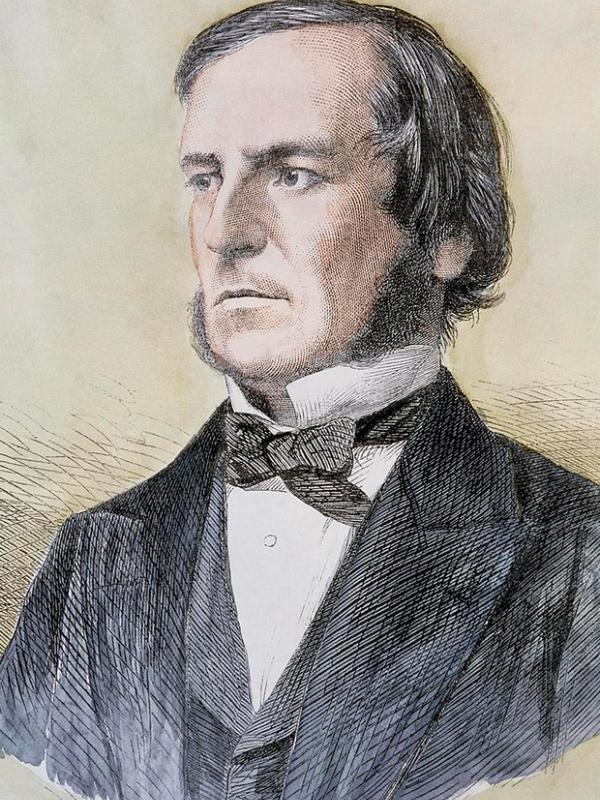
\includegraphics[width=0.3\linewidth]{George_Boole_color} \caption{A picture of George Boole}\label{fig:unnamed-chunk-26}
\end{figure}

Booleans are named after George Boole who was an English mathematician. He is notable for a few things including writing a book with the impressive title \emph{The Laws of Thought}. He also became a professor of mathematics at the university of Cork despite being largely self taught after primary school. His wife, Mary Everest Boole is also interesting and an example of a woman who made a career on the borders of academic mathematics when it was extremely hostile. Its worth looking them both up!

\begin{definition}[Boolean operator]
A Boolean operator is a function from \(f: \mathcal{B}^n \rightarrow \mathcal{B}\).

The value of \(n\) is called the \emph{arity} of \(f\).
\end{definition}

\begin{example}
There are some key examples of \emph{arity} 1 which we write by \(P\) and \(\neg P\).

\(P\) is the identity operator under which \(T \mapsto T\) and \(F \mapsto F\).

\(\neg P\) is the negation operator under which \(T \mapsto F\) and \(F \mapsto T\). We say that \(\neg P\) is true if \(P\) is false and \(\neg P\) is false if \(P\) is true.
\end{example}

\begin{example}
The operators of arity 2 are very helpful for understading what is going on. A first example is \(P \wedge Q\) or \(P\) and \(Q\). Under this function
\begin{align*}
(T,T) & \mapsto T, \\
(T,F) & \mapsto F, \\
(F,T) & \mapsto F, \\
(F,F) & \mapsto F.
\end{align*}

We have further \emph{basic} operators of arity two, these are \(P \vee Q\) (spoken \(P\) or \(Q\)), \(P \Rightarrow Q\) (spoken \(P\) implies \(Q\) ) of \(P \Leftrightarrow Q\) (spoken \(P\) is equivalent to \(Q\)).

We can express the way these functions work in a table
\begin{equation}
\begin{array}{cc|ccc}
P & Q & (P \vee Q) & (P \Rightarrow Q) & (P \Leftrightarrow Q)\\
\hline
T & T & T & T & T \\
T & F & T & F & F \\
F & T & T & T & F \\
F & F & F & T & T
\end{array}
\end{equation}
\end{example}

We can compose Boolean operators and rewrite them in various different ways

\begin{example}
The operator \(\neg (P \wedge Q)\) is given by
\begin{align*}
(T,T) \mapsto F,
(T,F) \mapsto T,
(F,T) \mapsto T,
(F,F) \mapsto T.
\end{align*}

The operator \((\neg P) \vee (\neg Q)\) is given by
\begin{align*}
(T,T) \mapsto F,
(T,F) \mapsto T,
(F,T) \mapsto T,
(F,F) \mapsto T.
\end{align*}

Therefore, \(\neg(P \wedge Q)\) and \((\neg P) \vee (\neg Q)\) are in some sense the same function. We can say \(\neg(P \wedge Q)=(\neg P) \vee (\neg Q)\).
\end{example}

More generally we have the following definition

\begin{definition}
We say two Boolean operators \(f\) and \(g\) or arity \(n\) are the same if they are equal as functions (they map the same elements to the same elements).

We call a way of writing a Boolean operator \(f\) in terms of the basic operators \(\neg, \wedge, \vee, \Rightarrow, \Leftrightarrow\) an \emph{expression} for \(f\).
\end{definition}

\begin{example}
Both \(P\) and \(P \wedge P\) are expressions for the identity operator.
\end{example}

\begin{theorem}
Every Boolean operator has an expression in terms of the basic operators.
\end{theorem}

We don't quite have all the technology to prove this. If you are curious you can get a sense of why this is true by working out how you would go from knowing it is true for all operators of arity two to knowing it is true for all operators of arity three.

We can actually do better than this

\begin{theorem}
Every Boolean operator has an expression in terms of \(\neg\) and \(\vee\)
\end{theorem}

\begin{proof}
First we check that we can express all our basic operations like this.

\begin{align*}
P \wedge Q &= \neg ( (\neg P) \vee (\neg Q)),\\
P \Rightarrow Q &= (\neg P) \vee Q, \\
P \Leftrightarrow Q &= (P \Rightarrow Q) \wedge (Q \rightarrow P)\\
&= \neg ( (\neg(P \Rightarrow Q)) \vee (\neg(Q \Rightarrow P))) \\
& = \neg ((\neg((\neg P) \vee Q)) \vee (\neg ((\neg Q) \vee P))).
\end{align*}

Now suppose that we have an expression for \(f\) in terms of our basic operations we can then replace all instances of \(\wedge, \Rightarrow, \Leftrightarrow\) by their expression in terms of \(\neg, \vee\) in exactly the way we have when expanding out the expression of \(P \Leftrightarrow Q\).
\end{proof}

\section{Boolean algebra}\label{boolean-algebra}

The basic Boolean operators interact with eachother in much the same way set operations do. We have the following results whose proofs are omitted.

\begin{lemma}

Suppose that \(P, Q, R\) are Booleans then we have the following about \(\vee\):

\begin{itemize}
\item
  \(P \vee T = T\) and \(P \vee F = P\),
\item
  \(P \vee (Q \vee R)) =(P\vee Q) \vee R\),
\item
  \(P \vee Q = Q \vee P\),
\item
  \((P \Rightarrow Q) = T\) if and only if \(P \vee Q = Q\),
\item
  \(P \vee P = P\).
\end{itemize}

\end{lemma}

\begin{lemma}

Suppose that \(P, Q, R\) are Booleans then we have the following about \(\wedge\):

\begin{itemize}
\item
  \(P \wedge T = P\) and \(P \wedge F = F\),
\item
  \(P \wedge (Q \wedge R)= (P\wedge Q) \wedge R\),
\item
  \(P \wedge Q = Q \wedge P\),
\item
  \((P \Rightarrow Q)= T\) if and only if \(P \wedge Q = P\),
\item
  \(P \wedge P = P\).
\end{itemize}

\end{lemma}

\begin{lemma}

Here are some distributive laws. Suppose that \(P, Q, R\) are Boolean's then

\begin{itemize}
\item
  \(P \wedge (Q \vee R) = (P \wedge Q) \vee (P \wedge R)\),
\item
  \(P \vee (Q \wedge R) = (P \vee Q) \wedge (P \vee R)\).
\end{itemize}

\end{lemma}

\begin{lemma}

And finally we get to De Morgan's law's again:
Suppose \(P\) and \(Q\) are Booleans then

\begin{itemize}
\item
  \(\neg (P \vee Q) = (\neg P) \wedge (\neg Q)\),
\item
  \(\neg (P \wedge Q) = (\neg P) \vee (\neg Q)\).
\end{itemize}

\end{lemma}

\begin{proof}
We give just one example of how you would prove such a statement

\begin{equation*}
\begin{array}{cc|ccccc}
P & Q & (P \vee Q) & \neg (P \vee Q) & \neg P & \neg Q & ((\neg P) \wedge (\neg Q)) \\
\hline
T & T & T & F & F & F & F\\
T & F & T & F & F & T & F\\
F & T & T & F & T & F & F\\
F & F & F & T & T & T & T \\
\end{array}
\end{equation*}

Observing that the fourth column \(\neg (P \vee Q)\) and the seventh column \(((\neg P) \wedge (\neg Q))\) are always the same proves that these expressions are the same as functions.
\end{proof}

\begin{definition}[tautologies]
If \(f: \mathcal{B}^n \rightarrow \mathcal{B}\) is a Boolean operator then we call \(f\) a \emph{tautology} if \(f(x) = T\) for all \(x \in \mathcal{B}^n\). We call \(f\) an \emph{antinomy} if \(f(x) = F\) for all \(x \in \mathcal{B}^n\).
\end{definition}

Tautologies are useful because they describe ways in which we can make logical arguments. For example, if we are arguing by contradiction (more on this later) we wish to prove \(P\). We assume \(\neg P\) and arise at a contradiction, so we know \(\neg P\) is false then we move from this to saying \(P\) must be true.

Here are some useful tautologies and their names

\begin{equation}
\begin{array}{lr}
\neg (\neg P) \Leftrightarrow P & \mbox{double negation elimination}\\
(P \Rightarrow Q) \Leftrightarrow ((\neg Q) \rightarrow (\neg P)) & \mbox{contraposition}\\
(P \Rightarrow Q) \Leftrightarrow ((\neg P) \vee Q) & \mbox{definition of implication}\\
(P \Leftrightarrow Q) \Leftrightarrow ((P \Rightarrow Q) \wedge (Q \Rightarrow P)) & \mbox{definition of equivalence}\\
(P \vee \neg P) & \mbox{law of the excluded middle}\\
(P \wedge (P \Rightarrow Q)) \Rightarrow Q & \mbox{modus ponens}\\
((P \Rightarrow Q) \wedge (Q \Rightarrow R)) \Rightarrow (P \Rightarrow R) & \mbox{transitivity of implication}\\
((\neg P)\Rightarrow F)\Rightarrow P & \mbox{argument by contradiction}
\end{array}
\end{equation}

\section{Truth tables}\label{truth-tables}

\begin{definition}[Truth tables]
A truth table is table which allows you to look up the output of a Boolean operator given its variables. Given a Boolean operator \(f\) of arity three the truth table will look like

\begin{equation}
\begin{array}{ccc|c}
P & Q & R & \mbox{an expression for \(f\)} \\
\hline
T & T & T & f(T,T,T)\\
T & T & F & f(T,T,F)\\
T & F & T & f(T,F,T)\\
T & F & F & f(T,F,F)\\
F & T & T & f(F,T,T)\\
F & T & F & f(F,T,F)\\
F & F & T & f(F,F,T)\\
F & F & F & f(F,F,F)
\end{array}
\end{equation}

We extend this in the way you would expect to Boolean operators of different arity. We also often evaluate more than one expression.

You have already seen a lot of truth tables in the previous section without me having given them a name.
\end{definition}

We often wish to compute truth tables by breaking expressions down to their constituent parts. For example if we want to check that the transitivity of implication is indeed a tautology we can do as follows

\begin{equation}
\begin{array}{ccc|ccccc}
P & Q & R & (P \Rightarrow Q) & (Q \Rightarrow R) & (P \Rightarrow R) & ((P\rightarrow Q)\wedge (Q\rightarrow P)) & (((P\rightarrow Q)\wedge (Q\rightarrow P))\\
 \, & \, & \, & \, & \, & \, & \, &\Rightarrow (P \Rightarrow R)) \\
\hline
T & T & T & T & T & T & T & T\\
T & T & F & T & F & F & F & T\\
T & F & T & F & T & T & F & T\\
T & F & F & F & T & F & F & T\\
F & T & T & T & T & T & T & T\\
F & T & F & T & F & T & F & T\\
F & F & T & T & T & T & T & T\\
F & F & F & T & T & T & T & T
\end{array}
\end{equation}

\section{Quantifiers}\label{quantifiers}

Quantifiers are \(\forall\) and \(\exists\) we want to start using these in our logical expressions.

We can use quantifiers to turn the sentence ``for all \(n \in \mathbb{N}\) there exists a \(p > n\) such that \(p\) is prime. First we define the function \(Prime: \mathbb{N} \rightarrow \{T, F\}\) by \(Prime(n) =T\) when \(n\) is prime, and \(F\) otherwise. Then we can write
\[\forall n (\exists p((p>n)\wedge(Prime(p)))).  \]
The order of quantifiers is very important
\[\exists p (\forall n ((p>n)\wedge (Prime(p))))  \] means that there exists a prime \(p\) that is bigger than every natural number \(n\). Which definitely isn't true.

\begin{remark}
When we are using quantifiers there is an ambient set sitting behind our language. We often surpress this set but in the previous expressions above we are always saying \emph{for all \(n\) in \(\mathbb{N}\)} and \emph{for every \(p\) in \(\mathbb{N}\)}.
\end{remark}

As with earlier we also have rules for negation and distribution with quantifiers.

\begin{lemma}

Quantifiers distribute as follows:

\begin{itemize}
\item
  \((\forall a \in A, S(a)\wedge T(a)) = (\forall a \in A, S(a))\wedge(\forall a \in A, T(a))\),
\item
  \(\exists a \in A, S(a)\vee T(a)) = (\exists a \in A, S(a))\vee (\exists a \in A, T(a))\).
\end{itemize}

We also have the negation rules:

\begin{itemize}
\item
  \(\neg(\forall a \in A, S(a))= (\exists a \in A, \neg S(a))\),
\item
  \(\neg(\exists a \in A, S(a)) = (\forall a \in A, \neg S(a))\).
\end{itemize}

\end{lemma}

As with earlier results these are fairly straightforward to prove just by writing out exactly what everything means.

\chapter{Proof}\label{proof}

Proof can be a difficult and subtle concept. During your first year you develop a good sense of proof by \emph{seeing lots of proofs}. In this section we will work towards a rigorous notion of what a proof is and study some common proof techniques.

First, to show this is really necessary let us look at some false proofs.

\begin{theorem}[untheorem]
\[e^i =1\]
\end{theorem}

\begin{proof}[unproof]
\[ e^i = (e^i)^{2\pi/2\pi} = (e^{2\pi i})^{1/2\pi} = 1^{1/2\pi} = 1.\]
\end{proof}

\begin{theorem}[untheorem]
All triangles are isoceles
\end{theorem}

\begin{proof}[unproof]

\begin{figure}
\centering
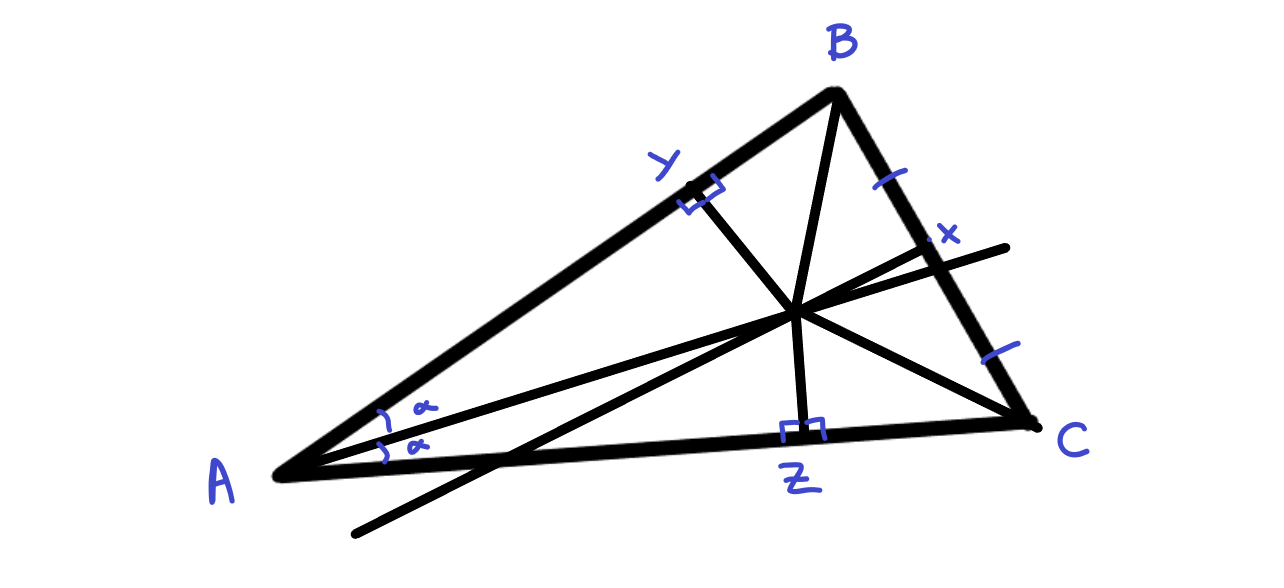
\includegraphics{badtriangle.png}
\caption{\label{fig:unnamed-chunk-27}A picture of a triangle}
\end{figure}

Consider the triangle \(ABC\). Draw the angle bisector at \(A\) and the perpendicular bisector of \(BC\). Call the point where these two intersect \(P\). Now draw a line from \(P\) to \(AB\) which is perpendicular to \(AB\) and call the intersection \(Y\) and draw a line from \(P\) to \(AC\) which is perpendicular to \(AC\) and call the intersection point \(Z\).

Now the triangles \(AYP\) and \(AZP\) are reflections of each other since they share two angles and a length. This means that the length \(AY\) is equal to the length \(AZ\) and the length \(YP\) is equal to \(ZP\).

Now the triangles \(BPX\) and \(APX\) are also reflections of each other since they both have right angles at \(X\) and share the two side lengths either side of the right angle. This implies that the lengths \(BP\) and \(CP\) are the same.

Then the triangles \(BPY\) and \(APZ\) are reflections of each other since they share two side lengths and a right angle. This means that the lengths \(BY\) and \(AZ\) are the same.

Now the length \(AB\) is equal to the lengths \(AY\) plus \(YB\) and the length \(AC\) is equal to the lengths \(AZ\) plus \(ZC\). Therefore \(AB = BC\).

\end{proof}

Can you spot the problems in the proofs above? If they didn't give obviously false results do you think you would notice that they were false.

\section{Patterns of proof}\label{patterns-of-proof}

In this section I am going to write proofs out using largely the language of logic. My hope is that it will make the different patterns of proof clear. In general it is neither necessary nor desirable to do this.

\begin{definition}
Proof by \emph{direct implication} is the most straightforward kind of proof. Here we want to prove \(P \Rightarrow Q\).
\end{definition}

\begin{example}
Suppose we want to prove that \(n\) being even implies that \(n^2\) is even. We can do this directly:

\begin{align*}
 & n \, \mbox{even} \, \Rightarrow \, \exists \, k \in \mathbb{N} \, s.t. n=2k, \\
 & n = 2k \, \Rightarrow \, n^2 = (2k)^2 = 2 (2k^2), \\
 & n^2 = 2(2k^2) \, \Rightarrow \, n^2 \, \mbox{even}.
\end{align*}

So you see we just flow from one implication to the next.
\end{example}

\begin{definition}
Proof by \emph{contraposition} is when we use the equivalence \((P\Rightarrow Q) \Leftrightarrow ((\neg Q) \Rightarrow (\neg P))\).
\end{definition}

\begin{example}
Suppose we want to prove that if \(n\) is odd then \(n^2\) is odd by contraposition. We need to use the following facts:

\begin{itemize}
\item
  (H1) If \(p\) is a prime and \(a,b \in \mathbb{N}\) then \(p|ab \, \Rightarrow (p|a)\vee(p|b)\).
\item
  (H2) 2 is a prime
\end{itemize}

We have:

\begin{align*}
& \neg (n^2 \, \mbox{odd}) \, \Rightarrow \, (n^2 \, \mbox{even}), \\
& (n^2 \, \mbox{even}) \, \Rightarrow \, (\exists \, k \in \mathbb{N} \, s.t. \, n^2=2k) \\
& ((n^2=2k)\wedge(H1)\wedge(H2))\, \Rightarrow \,(2|n)\\
& (2|n)\, \Rightarrow \, \neg(n \, \mbox{odd})\\
& ((\neg(n^2 \, \mbox{odd})) \Rightarrow (\neg(n \, \mbox{odd})) \Rightarrow ((n \, \mbox{odd})\Rightarrow (n^2 \, \mbox{odd}))
\end{align*}
\end{example}

\begin{definition}[proof by contradiction]
Proof by contradiction is when we use the fact that \((\neg P \Rightarrow F) \Rightarrow P\). So we assume the opposite of what we are trying to prove and get to a contradiction.
\end{definition}

\begin{example}
Suppose we want to prove there does not exist any \(r \in \mathbb{Q}\) such that \(r^2=2\).
Again first we need another results:

\begin{itemize}
\item
  We say \(p,q \in \mathbb{Z}\) are coprime if there is no prime number \(k\) such that \(k|p\) and \(k|q\). Let us write the function \(coprime: \mathbb{Z}^2 \rightarrow \{T,F\}\) to tell us if two numbers are coprime.
\item
  If \(r \in \mathbb{Q}\) then there exists \(p,q \in \mathbb{Z}\) with \(coprime(p,q) =T\) such that \(r=p/q\)
\end{itemize}

\begin{align*}
&\neg(\not\exists \, r \in \mathbb{Q} \, s.t. \, r^2 =2) \Rightarrow (\exists \, r \in \mathbb{Q} \, s.t. \, r^2 = 2)\\
&(\exists \, r \in \mathbb{Q} \, s.t. \, r^2 = 2) \Rightarrow (\exists \, p, q, \in \mathbb{Z} \, s.t. (p^2 = 2 q^2)\wedge((coprime(p,q)))) \\
&( p^2 = 2 q^2)  \Rightarrow (2|p^2) \Rightarrow (2|p) \\
& (\exists \, p, q, \in \mathbb{Z} \, (p^2 = 2 q^2)\wedge(2|p)) \Rightarrow (\exists \, k \in \mathbb{Z} s.t.\, p=2k)\wedge(4k^2=2q^2) )\\
&(4k^2=2q^2) \Rightarrow (2k^2 = q^2) \Rightarrow (2|q)\\
&((2|p)\wedge(2|q)\wedge (coprime(p,q))) \Rightarrow F\\
&\neg(\not\exists \, r \in \mathbb{Q} \, s.t. \, r^2 =2) \Rightarrow F
\end{align*}
\end{example}

\begin{definition}
Proof by construction. This method of proof is about showing that something exists.
\end{definition}

\begin{example}
Suppose we want to prove that every quadratic equation with integer coefficients has at least one solution in \(\mathbb{C}\). i.e.~we want to show if \(a,b,c \in \mathbb{Z}\) then the equation \[ ax^2+bx+c = 0 \] has at least one solution. We can check (and I'm sure you have before) that
\[ x = \frac{-b\pm \sqrt{b^2-4ac}}{2a},  \] is a solution. So we have demonstrated the existence of at least one solution.

Another good example of proof by construction is the proof of Cantor-Schroeder-Bernstein.
\end{example}

\section{Proof by induction}\label{proof-by-induction}

A particularly important pattern of proof is \emph{proof by induction}. Induction is a key property of how the natural numbers work.

\begin{definition}[proof by induction]
Suppose that \(P\) is a property that could or could not hold for each natural number. We can think of \(P\) as a function \(\mathbb{N}\rightarrow \{T,F\}\). Suppose the following hold

\begin{itemize}
\item
  \(P(0)=T\) (alternatively we say \(P(0)\) holds) - this is called the base case,
\item
  \(\forall \, n \in \mathbb{N} \, P(n) \Rightarrow P(n+1)\) - this is called the inductive step,
\end{itemize}

then we can conclude that \(P(n)\) holds for every \(n\). We can write this as \(\forall n \in \mathbb{N} \, P(n)\).
\end{definition}

\begin{remark}
Proof by induction works equivalently (by relabling things) if we start at \(n=1\) or in fact from any number \(k\) we just have to alter the conclusion to say \(\forall n \geq k \, P(n)\).
\end{remark}

\begin{example}
Let \(P(n)\) be the statement that the sum of the first \(n\) odd numbers is \(n^2\).

Base case: For \(n=1\) the sum of the first odd number is \(1 = 1^2\).

Inductive step: Suppose that \[ \sigma_{k=1}^n (2k-1) = n^2 \] then
\[ \sigma_{k=1}^{n+1} (2k-1) = n^2 + 2(n+1) -1 = n^2 +2n +1 = (n+1)^2.  \] So we have shown \(P(n) \Rightarrow P(n+1)\).

Therefore we have shown \(P(n)\) holds for all \(n \geq 1\).
\end{example}

\begin{definition}[well ordering principle]
Suppose that \(S \subset \mathbb{N}\) and \(S \neq \emptyset\) then \(S\) has a \emph{smallest element}.
\end{definition}

A classic example of using the well ordering principle is the prime factorisation theorem.

\begin{theorem}[prime factorisation]
Every \(n \in \mathbb{N}-\{0\}\) is the product of prime factors.
\end{theorem}

\begin{proof}
Let C be the set of all natural numbers that aren't the product of prime factors. We want to show \(C\) is empty.

We assume for contradiction that \(C \neq \emptyset\) then by the well ordering principle \(C\) has a least element. Let us call this element \(m\).

If \(m\) only has divisors \(1\) and \(m\) then \(m\) is prime so is the product of prime factors which would be a contradiction.

If \(m\) has another divisor \(k \neq 1,m\) then we must have \(m=kj\) for some \(k, j \in \mathbb{N}-\{0\}\). This implies \(k, j < m\) so both \(k\) and \(j\) are the product of prime factors. This implies \(m\) is the product of prime factors which is a contradiction.

Therefore \(C\) must be empty.
\end{proof}

\begin{definition}[strong induction]
Suppse \(P\) is a property that could or could not hold for each of the natural numbers. Suppose that the following are true.

\begin{itemize}
\item
  \(P(0)\) holds,
\item
  If \(P(k)\) holds for all \(k<n\) then \(P(n)\) holds,
\end{itemize}

then we can conclude that \(P(n)\) holds for all \(n \in \mathbb{N}\).
\end{definition}

\begin{theorem}[unique prime factorisation]
Every natural number \(n \geq 2\) has a \emph{unique} prime factorisation.
\end{theorem}

\begin{proof}
In this proof we are going to assume the fact that if \(p\) is a prime and \(p|ab\) then \(p|a\) or \(p|b\). If you are doing ma132 you will see this proved later.

For the base case \(2\) has a unique prime factorisation.

Suppose that for every \(k < n\) that \(k\) has a unique prime factorisation.

We already know that \(n\) has a prime factorisation from the prime factorisation theorem. It remains to show that it is unique.

Suppose that there are two prime factorisations

\[ n=p_1\dots p_k = q_1 \dots q_j.  \]

By re-ordering we can assume that \(p_1 \leq p_2 \leq \dots\) and \(q_1 \leq q_2 \leq \dots\).

If \(p_1=q_1\) then \(n/p_1\) has a unique prime factorisation so we must have \(p_2=q_2\) etc.

If \(p_1 \neq q_1\) then without loss of generality \(p_1 < q_1\).

\[ p_1p_2 \dots p_k - p_1 q_2 q_3 \dots q_j = n (1-p_1/q_1) = (q_1-p_1)q_2\dots q_n.\]

If we call \(m = (q_1-p_1)q_2 \dots q_n\) then the expression on the left tells us that \(p_1|m\) and the expression on the right tells us that \(m < n\) since \(q_1-p_1 < q_1\). Therefore \(m\) has a unique prime factorisation and \(p_1|m\). We know that \(q_k > p_1\) for all \(k\) so we must have \(p_1|(q_1-p_1)\) but this would imply that \(p_1|q_1\) which is a contradiction to \(q_1\) being prime with \(p_1<q_1\). So we cannot have \(p_1 \neq q_1\).
\end{proof}

\begin{theorem}
Induction, the well ordering principle and strong induction are all equivalent.
\end{theorem}

\begin{proof}
(Induction \(\Rightarrow\) Well ordering principle): Given a set \(S \subset \mathbb{N}\) let us assume that \(S\) has no least element. Then let \(P(n)\) be the property than \(S \cap [[n]]= \emptyset\).

If \(0 \in S\) then \(0\) would be the least element of \(S\) so \(S \cap [[0]]= \emptyset\). This is the base case.

If \([[n]] \cap S = \emptyset\) then if \(n+1 \in S\) then \(n+1\) would be the least element of \(S\) so \([[n+1]] \cap S = \emptyset\).

Therefore induction implies that \(S = \bigcup_n (S \cap [[n]])\) is empty.

(Well ordering principle \(\Rightarrow\) strong induction):

Suppose that the well ordering principle holds and we have a property \(P\) such that \(P(0)\) holds and for every \(n\), \((P(k) \forall k<n) \Rightarrow P(n)\). Then set \(S\) be the set where \(P\) doesn't hold. If \(S \neq \emptyset\) by well ordering it has a least element \(m\). By definition of \(S\) we must have \(P(k)\) holding for all \(k<m\) therefore we must have \(P(m)\) holds. This shows that \(S\) must be empty so \(P(n)\) holds for all \(n\).

(Strong induction \(\Rightarrow\) induction):

Suppose that strong induction holds and we have some property \(P\) such that \(P(0)\) holds and \(P(n) \Rightarrow P(n+1)\) for all \(n\). Then we also have \(P(k) \forall k< n \Rightarrow P(n)\) since \(P(k) \forall k < n \Rightarrow P(n-1) \Rightarrow P(n)\) so by strong induction \(P(n)\) holds for all \(n\).
\end{proof}

\chapter{Some number theory}\label{some-number-theory}

\section{Divisors and prime numbers}\label{divisors-and-prime-numbers}

Let us recall the definition of divisor and prime numbers

\begin{definition}[divisor]
Given two natural numbers \(n\) and \(m\) we say \(n\) is a divisor of \(m\) (or \(n|m\)) if there exists \(k \in \mathbb{N}\) such that \(m=n\times k\).
\end{definition}

\begin{definition}[prime number]
While we define divisor it is worth defining a prime number. We call \(p \in \mathbb{N}\) a \emph{prime number} if the only divisors of \(p\) are \(1, p\).
\end{definition}

Now we have some new definitions

\begin{definition}[greatest common divisor]
Given two natural numbers \(n\) and \(m\) a number \(q\) that divides both of them is a common divisor and the largest such number is called the \emph{greatest common divisor} we write \(gcd(n,m)\).
\end{definition}

This allows us to write a better definition of coprime

\begin{definition}[coprime]
If \(gcd(n,m)=1\) then \(n\) and \(m\) are coprime.
\end{definition}

\begin{theorem}[division with remainder]
Suppose that \(a \in \mathbb{Z}, b \in \mathbb{N}-\{0\}\) then there exists \(q \in \mathbb{Z}\) and \(r \in [[b]]\) such that
\[ a =bq+r.  \]
\end{theorem}

\begin{proof}
If \(b=1\) we just take \(q=a, r=0\) so we can work in the case \(b >1\).

Let us fix \(b\) and prove the result by induction on \(a\). If \(a=1\) then \(a=0\times b+1\). This is the base case.

Now if we assume that there exists \(q,r\) such that \(a-1 = qb +r\) then either \(r \in [[b-1]]\) in which case \(a = qb + (r+1)\) is a solution to our problem, or \(r=b-1\) in which case we write \(a = (q+1)b\).
\end{proof}

\begin{example}
How can we find the greatest common divisor of two numbers. One way to do it is by repeated division.

We can apply repeated division with \(81\) and \(51\). We have
\begin{align*}
81 & = 1 \times 51 + 30,\\
51 & = 1 \times 30 + 21,\\
30 & = 1 \times 21 + 9,\\
21 & = 2 \times 9 + 3,\\
9 & = 3 \times 3.
\end{align*}

We can also do this backwards to get
\begin{align*}
9 & = 3 \times 3,\\
21 & = 2 \times 9 + 3 = (2 \times 3 +1) \times 3 = 7 \times 3,\\
30 & = 1 \times 21 + 9 = (1 \times 7 + 3) \times 3 = 10 \times 3,\\
51 & = (1 \times  10 + 7) \times 3 = 17 \times 3,\\
81 & = (1 \times 17 + 10) \times 3 = 27 \times 3.
\end{align*}

And we deduce from the that \(gcd(81,51) = 3\).

Why does this work? We notice that if \(c|a, c|b\) then if \(a=qb+r\) then we must have that \(c|r\). Continuing on if \(c|b\) and \(c|r\) and \(b=q_2 r+ r_2\) then \(c|r_2\) and so on. If eventually you end up with a remainder term which is 0 then we terminate. This shoes that if we terminate with remainder \(r_k\) then \(r_k|a\) and \(r_k| b\) and that nothing larger than \(r_k\) can divide both \(a\) and \(b\).
\end{example}

\section{Euclid's Algorithm}\label{euclids-algorithm}

Taking inspiration from calculations like the one above we can write down a procedure to find the greatest common divisor of \(a,b\).

\begin{definition}[Euclid's Algorithm]
Given \(a, b \in \mathbb{N}\) with \(a < b\) we can write
\begin{align*}
b &= q_1a + r_1, \quad q_1 \in \mathbb{N}, r_1 \in [[a]],\\
a &= q_2r_1 + r_2, \quad q_2 \in \mathbb{N}, r_2 \in [[r_1]],\\
r_1 &= q_3r_2 + r_3, \quad q_3 \in \mathbb{N}, r_3 \in [[r_2]],\\
r_2 & = \dots
\end{align*}
Eventually this process will terminate because we will have \(r_k = 0\) for some \(k\) and then we have \(r_{k-1} = gcd(a,b)\).
\end{definition}

\begin{theorem}[Euclid's Algorithm]
Given the algorithm above we have the following
- This algorithm will terminate. i.e.~eventually we have \(r_{k-1} = q_{k+1} r_{k} + 0\).
- In this case \(r_{k} = gcd(a,b)\)
- There exists \(x,y \in \mathbb{Z}\) such that \(gcd(a,b) = xa+by\).
\end{theorem}

\begin{proof}
We take each point in turn.

Firstly we can see that, for every \(j\), \(r_j> r_{j+1} > r_{j+2}\) so eventually we must get to 0. Therefore the sequence terminates.

Secondly, we prove this by showing that in each step of the algorithm we preserve the set of common divisors. If \(m|r_j\) and \(m|r_{j+1}\) then since \(r_j = q_{j+2}r_{j+1} + r_{j+2}\) so \(m|r_{j+2}\) as well. Equally if \(n|r_{j+1}\) and \(n|r_{j+2}\) then we must have \(n|r_j\) as well. So the set of divisors of \(r_j, r_{j+1}\) is the same as the set of divisors of \(r_{j+1},r_{j+2}\). From this it follows that \(gcd(r_j,r_{j+1})=gcd(r_{j+1},r_{j+2})\). Therefore itterating backwards we have that for every \(j\) that \(gcd(r_j, r_{j+1}) = gcd(a,b)\). Consequently at the point where the algorithm terminates, \(r_k = gcd(r_k,0)=gcd(r_k,r_{k+1})=gcd(a,b)\).

For the last point let us make the claim: For every \(j\) we can write \(r_j = x_j a + y_j b\) for some \(x_j, y_j \in \mathbb{Z}\). Then we can prove this recursively. First we know that \(b=q_1 a + r_1\) so \(r_1 = -q_1 a + 1*b\). Now suppose that \(r_{j-1}, r_{j-2}\) can be expressed as above. We know \(r_{j-2} = q_j r_{j-1} + r_j\) so \(r_j = r_{j-2} - q_j r_{j-1} = x_{j-2} a + y_{j-2} b - q_j(x_{j-1}a + y_{j-1}b) = (x_{j-2}-q_j x_{j-1})a + (y_{j-2} - q_j y_{j-1})b\). So this shows the claim by induction. Now the claim implied in particular that \(r_k = x_k a + y_k b\) proving the third point in the theorem.
\end{proof}

\subsection{Geometric interpretation of Euclid's algorithm}\label{geometric-interpretation-of-euclids-algorithm}

We can think of this algorithm pictorially by drawing a rectangle of length \(a\) and height \(b\) and then \(q_1\) squares of side length \(b\) inside it leaving a rectangle of length \(r_1\) and height \(b\) and so on\ldots{}

\begin{figure}
\centering
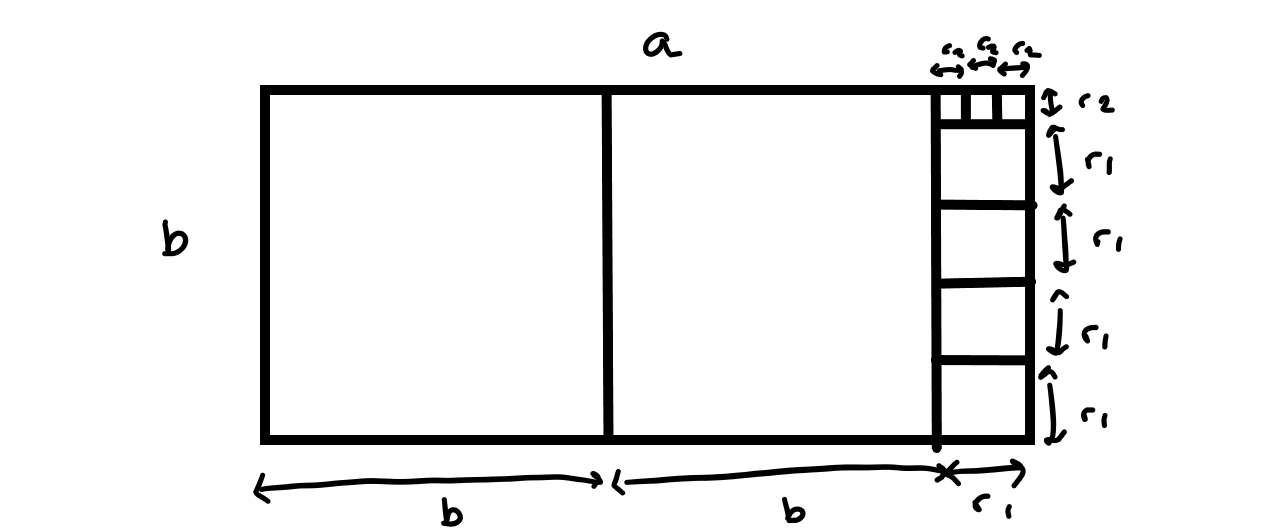
\includegraphics{geomeuclid.png}
\caption{\label{fig:unnamed-chunk-28}Picture showing Euclid's algorithm pictorially}
\end{figure}

Here is a specific example with the numbers \(24\) and \(15\)

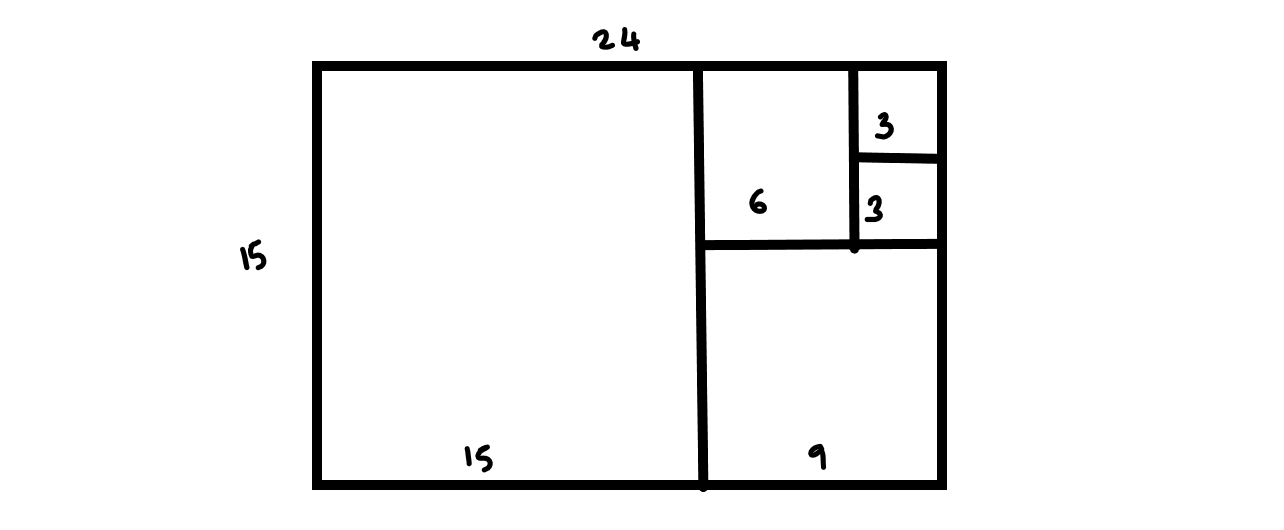
\includegraphics{geomeuclidnumbers.png}
\#\#\# Continued fractions

Another way of looking at Euclid's algorithm is continued fractions. If \(a = qb+r\) then
\[ \frac{a}{b} = q + \frac{r}{b}.  \]
If \(b = q_2 r + r_2\) then
\[  \frac{b}{r} = q_2 + \frac{r_2}{r},\] so
\[ \frac{a}{b} = q + \frac{1}{q_2 + \frac{r_2}{r}}.  \]
Continuing on like this we can express
\[ \frac{a}{b} = q + \frac{1}{q_2 + \frac{1}{q_3 + \dots}}.  \]

In a similar way if we take some real number \(x\) we can write it in continued fraction form by writing \(q_1 = [x]\) and \(q_2 = [1/(x-[x])]\) and so on. Unlike when expressing a rational number this process might not terminate.

In both situations we call this the continued fraction representation of a number.

\subsection{Bezout's lemma}\label{bezouts-lemma}

The final statement in Euclid's algorithm is called Bezout's lemma

\begin{lemma}[Bezout's Lemma]
If \(a,b\) are two natural numbers then there exists \(x,y \in \mathbb{Z}\) such that
\[ gcd(a,b) = x a + b c.  \]

As a result of this if \(a,b\) are coprime and \(n\) is any integer then there exists \(x, y \in \mathbb{Z}\) such that
\[ n = xa + yb.\]
\end{lemma}

\begin{proof}
We have already proved the first part in the discussion of Euclid's algorithm.

For the second if \(a,b\) are coprime then \(gcd(a,b) =1\) (this is the definition of being coprime). Then by the first part of the theorem there exists \(\tilde{x}, \tilde{y} \in \mathbb{Z}\) such that
\[ 1= \tilde{x}a + \tilde{y}b,  \] using this
\[ n = (n\tilde{x})a + (n \tilde{y})b.  \]
\end{proof}

Using this we can show a powerful result which we have already seen

Suppose that \(a,b \in \mathbb{N}\) and \(p\) is a prime number and \(p|ab\) then either \(p|a\) or \(p|b\).

If \(p|a\) then we are done so suppose that \(p\) does not divide \(a\). Then \(a,p\) are coprime so by Bezout's lemma we can write
\[1 = xa + yp\] and hence
\[b = xab + ypb.  \] As \(p|ab\) we know \(p|xab\) and from the expression we can see that \(p|ypb\) so \(p | (xab + ybp)\) so \(p|b\).

Now let us use this to prove the fundamental theorem of arithmetic again. Everything is a bit smoother now with more results.

\begin{theorem}[Fundamental Theorem of Arithmetic]
Any natural number \(n\) has a unique factorisation into prime numbers.
\end{theorem}

\begin{proof}
First let us use strong induction to prove that there is a prime factorisation. The base case is \(n=2\) which is already in prime factorisation. Now suppose that every number less than \(n\) can be written as a product of prime factors. Then either \(n\) is prime, so it is in prime factorisation or \(n=ab\) then \(a,b < n\) so they have prime factorisations which allows us to write a prime factorisation for \(n\).

Second we want to prove this factorisation is unique. Suppose \(n = p_1 p_2 \dots p_k = q_1 q_2 \dots q_j\) where all the \(p_i, q_i\) are primes. Then \(p_1 | n\) so \(p_1|q_1\) or \(p_1 |q_2\dots q_j\). In the first case we must have \(p_1=q_1\) since \(q_1\) is prime. In the second case we have \(p_1|q_2\) or \(p_1 |q_3 \dots q_j\) and so on. We can keep itterating to show that \(p_1\) must appear in the list \(q_1, \dots q_j\). We can then repeat this with all the \(p_i\).
\end{proof}

\section{Chinese remainder theorem}\label{chinese-remainder-theorem}

Suppose we are interested in solving two or more linear congruences simultaneously.

\begin{example}
Suppose we would like to find \(x\) such that \(x \equiv 1 \quad \mbox{mod} \, 3\) and \(x \equiv 3 \quad \mbox{mod} \, 4\). Then we can work modulo 12 since if we have a solution we can see we will get another solution by adding multiples of 12. If \(x \equiv 1 \quad \mbox{mod} \, 3\) then modulo 12 \(x \equiv 1, 4, 7\) or \(10\). Similarly, if \(x \equiv 3 \quad \mbox{mod}\, 4\) then \(x \equiv 3, 7\) or \(11\) modulo 12. Therefore \(x \equiv 7\) modulo 12 is our unique solution up to adding multiples of 12.

Slightly differently suppose we would like to have \(x \equiv 2 \quad \mbox{mod} \, 6\) and \(x \equiv 3 \quad \mbox{mod} \, 4\) then again we want to work modulo 12. From the first constraint we have \(x \equiv 2\) or \(x \equiv 8\) and from the second we have \(x \equiv 3, 7\) or \(11\) as before. In this example we see there are no possible solutions.
\end{example}

\begin{theorem}[Chinese Remainder Theorem]
Suppose that \(n_1, \dots, n_k\) are pairwise coprime integers and \(a_1, \dots, a_k\) are integers with \(a_i \in [[n_i]]\) for every \(i\). Then there exists an integer \(x\) with
\[ x \equiv a_i \quad \mbox{mod} n_i, \quad i = 1, \dots, k.  \] Furthermore all the solutions are equivalent modulo \(N=n_1 \dots n_k\).
\end{theorem}

\begin{proof}
Let \(m_i = \Pi_{j \neq i} n_j\). Then \(n_i\) and \(m_i\) are coprime so by Euclid's algorithm there exists \(x_i,y_i\) such that \(1 = x_i n_i + y_i m_i\) so \(e_i =y_i m_i = 1- x_i n_i\) so \(e_i \equiv 1 \quad \mbox{mod} \, n_i\) and \(e_i \equiv 0 \quad \mbox{mod} \, n_j\).

Then let \(x = \sum_{i=1}^k a_i e_i\) then this satisfies the conditions of the theorem.

Now suppose we have another \(y\) satisfying the congruences. Then \(x \equiv y \quad \mbox{mod} \, n_i\) for every \(i\). Therefore, \(n_i| |x-y|\) for every \(i\). Since all the \(n_i\) are coprime this means that \(N | |x-y|\).
\end{proof}

\begin{remark}
The Chinese remainder theorem is very old. It dates back to Sunzi in the 3rd to 5th Century. It can be used to do apparently complicated computations very quickly and is used in important algorithms today such as RSA cryptography and Fast Fourier transform.
\end{remark}

\section{Fermat's Little Theorem and Euler's Theorem}\label{fermats-little-theorem-and-eulers-theorem}

\begin{definition}
A number \(a\) is called a emph\{unit\} modulo \(n\) if there exists \(b\) such that \(ab = 1 \quad \mbox{mod} \, n\). (We call \(b\) a multiplicative inverse modulo \(n\).)
\end{definition}

\begin{lemma}
A number \(a\) is a unit modulo \(n\) if and only if \(a\) and \(n\) are coprime.
\end{lemma}

\begin{proof}
If \(a\) and \(n\) are coprime then \(1 = xa + yn\) in which case \(xa\equiv 1 \quad \mbox{mod} \, n\).

If there exists \(x\) such that \(xa \equiv 1 \quad \mbox{mod} \, n\) then \(x a = 1 + y n\) and \(gcd(a,n) | (xa-yn)\) so \(gcd(a,n) = 1\).
\end{proof}

\begin{definition}[Euler Totient Function]
The Euler Totient function \(\phi(n)\) counts the number of natural numbers smaller than \(n\) that are coprime to \(n\). Alternatively the number of units modulo \(n\). Notice that \(\phi(1)=1\).
\end{definition}

\begin{lemma}
If \(p\) is prime then \(\phi(p) = p-1\).
\end{lemma}

\begin{example}
Another example is \(n=12\) the numbers smaller than \(n\) which are coprime are \(1,5,7,11\) so \(\phi(12)=4\)
\end{example}

\begin{lemma}
If \(p\) is a prime then
\[ \phi(p^k) = p^k - p^{k-1}. \]
\end{lemma}

\begin{proof}
The only way that \(gcd(m,p^k) \neq 1\) is if \(m\) is a multiple of \(p\). There are \(p^{k-1}\) multiples of \(p\) less than \(p^k\).
\end{proof}

\begin{lemma}
If \(n\) and \(m\) are coprime integers then
\[ \phi(nm) = \phi(n)\phi(m). \]
\end{lemma}

\begin{proof}
Recall that the units modulo \(n\) are exactly the numbers which are coprime to \(n\). Let us write the set of units modulo \(n\) as \(\left(\mathbb{Z}/n \mathbb{Z} \right)^{\times}\).

Suppose that \(k\) is a unit modulo \(n\) and \(j\) is a unit modulo \(m\) then by the Chinese remainder theorem there exists a unique \(l\) such that \(l \equiv k \quad \mbox{mod} \, n\) and \(l \equiv j \quad \mbox{mod} \, m\). Equally if \(l\) is a unit modulo \(mn\) then there is some \(q\) such that \(lq \equiv 1 \quad \mbox{mod}\, mn\) so \(l\) is a unitt modulo \(n\) and a unit modulo \(m\). This shows we have a bijection between \(\left(\mathbb{Z}/n \mathbb{Z} \right)^{\times} \times \left(\mathbb{Z}/m \mathbb{Z} \right)^{\times}\) and \(\left(\mathbb{Z}/nm \mathbb{Z} \right)^{\times}\). Therefore the two sets have the same size. This gives our conclusion.
\end{proof}

\begin{proposition}
We have a formula for Euler's totient function given by
\[ \phi(n) = n \Pi_{p \, prime, p|n} (1-1/p).  \]
\end{proposition}

\begin{proof}
This follows from our previous results. By the fundamental theorem of arithmetic we can write \(n = p_1^{k_1} \dots p_j^{k_j}\) then
\begin{align*} \phi(n) &= \phi(p_1^{k_1}) \dots \phi(p_j^{k_j})  \\
& = p_1^{k_1}(1-1/p_1) \dots p_j^{k_j}(1-1/p_j) \\
& = n (1-1/p_1) \dots (1-1/p_j).
\end{align*}
\end{proof}

\begin{theorem}[Divisor sum]
If \(n\) is an integer then
\[ n = \sum_{d|n} \phi(d)  \]
\end{theorem}

\begin{proof}
We prove this by strong induction. We can see that it is true when \(n=1\) then the only divisor of 1 is itself and \(\phi(1) =1\). This gives us the base case.

For the inductive step we assume that for all \(m < n\) we have
\[ m = \sum_{d|m} \phi(d).  \]

Then there are two cases. If \(n\) is prime then \(n = n-1 +1 = \phi(n) + \phi(1)\) and we are done.

If \(n\) isn't prime then \(n=pm\) where \(p\) is prime and \(m < n\). From this we can compute:
\begin{align*} \sum_{d|n} \phi(d) &=  \sum_{d|m} (\phi(d)+\phi(pd))  \\
& = \sum_{d|m} \phi(d)(1 + \phi(p))\\
&= \sum_{d|m} \phi(d) p\\
& = p m = n. 
\end{align*}
\end{proof}

\begin{proposition}
If \(p\) is prime and \(a\) is not a multiple of \(p\) then
\[ a^{p-1} \equiv 1 \quad \mbox{mod} \, p.  \]
\end{proposition}

\begin{proof}
Let us consider \(a, 2a, 3a, \dots, (p-1)a\) as elements in \(\mathbb{Z}/p\mathbb{Z}\). We claim that they are all distinct. This is because since \(a,p\) are coprime, there exists \(x\) such that \(xa =1\) modulo \(p\). So if \(ka \equiv ja \quad, \mbox{mod} \,p\) then \(kab \equiv jab \quad \mbox{mod} \, p\) so \(k \equiv j \quad \mbox{mod}\, p\). So if \(k, j \in [[p]]\) this would imply \(k = j\).

So \(a, 2a, \dots, (p-1)a\) considered modulo \(p\) must be \(1, 2, \dots, (p-1)\) in some order. Hence
\[ a \times 2a \times \dots \times (p-1)a \equiv (p-1)! \quad \mbox{mod}\, p. \] Which rewriting is
\[ a^{p-1} (p-1)! \equiv (p-1)! \quad \mbox{mod} \, p. \] Now \((p-1)!\) is coprime to \(p\) since \(p\) is prime. So there exists \(c\) such that \(c(p-1)! \equiv 1 \quad \mbox{mod}\, p\) hence multiplying the equation above by \(c\) we get
\[ a^{p-1} \equiv 1 \quad \mbox{mod} \, p.  \]
\end{proof}

\begin{theorem}[Fermat's Little Theorem]
Suppose that \(gcd(a,n) =1\) then \(a^{\phi(n)-1} \equiv 1 \quad \mbox{mod} \, n\).
\end{theorem}

\begin{proof}
The proof is very similar to above so I will leave the details to you!

Consider the set of integers \{ka\} where \(gcd(k,n) =1\) and \(k \in [[n]]\) and multiply them all together.
\end{proof}

\begin{definition}[primitive root]
We say \(a\) is a \emph{primitive root} modulo \(n\) if for every \(b \in \mathbb{Z}/n\mathbb{Z}\) with \(gcd(b,n)=1\) there exists an \(x\) such that \(b \equiv a^x \quad \mbox{mod}\, n\).
\end{definition}

You have hopefully seen in Algebra 1 that \((\mathbb{Z}/n\mathbb{Z})^{\times}\) is the set of elements in \(\mathbb{Z}/n\mathbb{Z}\) which have multiplicative inverses. This set forms a group under multiplication and the primitive roots are the generators of this group.

\begin{example}
Working modulo \(5\) the primitive roots are \(2,3\) we can see that \(4^2 = 1\) which means it cannot be a primitive root.
\end{example}

\begin{lemma}
Suppose that \(p\) is prime and \(r|p-1\) then there are exactly \(r\) elements, \(b\), of \(\left(\mathbb{Z}/p\mathbb{Z} \right)^{\times}\) with \(b^r \equiv 1 \quad \mbox{mod}\, p\).
\end{lemma}

\begin{proof}
This is straightforward once you can talk about polynomials modulo \(p\) but we don't want to talk about it so we're leaving it unproved.
\end{proof}

\begin{proposition}
If \(p\) is prime and there exists an element \(a\) of order \(r\) then there are exactly \(\phi(r-1)\) elements of order \(r\).
\end{proposition}

\begin{proof}
Give an element \(a\) of order \(r\) then we have distinct elements \(a, a^2, \dots, a^{r-1}\). There are at most \(r\) elements \(b\) such that \(b^r \equiv 1 \quad \mbox{mod}\, p\) so these are all the possible elements of order less than or equal to \(r\). Now if \(gcd(k,r-1) = 1\) then for every \(m < r-1\) we have \(mk \not\equiv 0 \quad \mbox{mod} \, r-1\) so \(a^{mk} \not\equiv 1 \quad \mbox{mod} \, p\). However \(a^{rk} \equiv 1 \quad \mbox{mod} \, p\). Therefore \(a^k\) is another element of order \(r\). Therefore we have at least \(\phi(r-1)\) elements of order \(r\).
\end{proof}

\begin{corollary}
If \(p\) is prime then there are exactly \(\phi(p-1)\) primitive roots.
\end{corollary}

\begin{proof}
We know that the total number of elements in \(\left(\mathbb{Z}/p\mathbb{Z} \right)^{\times}\) is \(\sum_{r} \mbox{number of elements of order}\, r\). We also know that the size of \(\left(\mathbb{Z}/p\mathbb{Z} \right)^{\times}\) is \(p-1\) and so there can only be elements of order \(r\) if \(r|p-1\).

We also know know that \(p-1 = \sum_{d|p-1} \phi(d)\). Putting all this together gives our result.
\end{proof}

\chapter{Algorithms and Algorithmic complexity}\label{algorithms-and-algorithmic-complexity}

\section{Algorithmic Complexity}\label{algorithmic-complexity}

Algorithmic complexity is a measure of how complicated a procedure is by counting roughly how many operations are required to complete it.

\subsection{Big and little O notation}\label{big-and-little-o-notation}

When we are talking about complexity (and in lots of other situations later in your degree) we are often only interested in the asymptotic behaviour of a function.

For example if we want to know the complexity of an algorithm to multiply two numbers with at most \(n\) digits together we have a function of \(n\) and we are only really interested in describing how it behaves when \(n\) is very large. Big and little O notation is a way of doing this.

\begin{definition}[Big O]
Suppose \(f(n)\) and \(g(n)\) are function of \(n\) and there exist real numbers \(C, n_0\) such that for \(n \geq n_0\) then
\[|f(n)| \leq C g(n)\] then we say
\[ f(n) = O(g(n)).  \]
\end{definition}

This is most commonly used when \(g(n)\) is a simple function like \(n^k\) for some \(k\) or \(\log(n)\) or \(a^n\) or something similar.

\begin{example}

\begin{itemize}
\item
  The function \(2n^3 + 3n - 102 = O(n^3)\).
\item
  \(\phi(n) = O(n)\) since \(\phi(n) \leq n\).
\end{itemize}

\end{example}

While we are defining big O notation it is useful to define little o notation

\begin{definition}[little o notation]
If \(f(n), g(n)\) are functions and for every \(c >0\) there exists \(n_c\) such that if \(n >n_c\) then
\[ |f(n)| \leq c g(n).\]

We can think of this as saying \(f(n)\) becomes insignificant compared to \(g(n)\) as \(n\) becomes large.
\end{definition}

\begin{example}
We have \(n^2 = o(n^3)\).
\end{example}

\section{Running times of algorithms}\label{running-times-of-algorithms}

We use big O notation to talk about how long it will take to run an algorithm as the input becomes large. It is easiest to understand this by looking at some examples.

\begin{example}[Addition]
Suppose we are adding two \(n\) digit numbers \(a_1\dots a_n\) and \(b_1\dots b_n\) using our standard method of addition where we do \(a_n+b_n\) and enter the unit part of this as the unit part of the sum then possibly carry the 1 if \(a_n + b_n \geq 10\). Then we add \(a_{n-1} + b_{n-1}\) and possibly add the additional \(1\) we carried if necessary.

If we want to count the steps it depends on precisely what we list as a step. If we only think we are doing 1 step when adding and carrying for each place value then we are performing \(n\) steps. If we think of each addition and carrying step as a separate step then we do \(3n\) steps. However in either case we say the algorithm is \(O(n)\).
\end{example}

\begin{example}[Multiplication]
Now suppose we think about multiplication using the long multiplication algorithm then for two \(n\) digit numbers we need to multiply \(a_k\) by \(b_j\) for each \(k, j\) (which is \(n^2\) steps) and then perform \(n^2\) addition steps of what are effectively at most two digit numbers. So this algorithm is O(n\^{}2).
\end{example}

\begin{example}[Checking divisibility]
Division is no worse than multiplication. The algorithms are a bit more complicated to state. One example is given an \(n\) digit number, \(a\) and an \(m\) digit number, \(b\) with \(m\leq n\) and we want to know whether \(b|a\) then if \(a/b\) were an integer it would have at most \(n-m+1\) digits and at least \(n-m\). So we are have around \(20\) possible candidate for \(a/b\). Now we just check multiplying all \(20\) candidates with \(m\) which is a multiplication operation with \(m\times(n-m+1)\) steps so \(O(n^2)\) and we do this 20 times so checking divisibility is \(O(n^2)\).
\end{example}

\begin{example}[Naive primality testing]
Suppose we want to test whether a number \(n\) is prime. The most obvious way to do this is to check whether we can find any other \(m \neq n\) such that \(m|n\). We notice here that we only need to check \(m \leq \sqrt{n}\) as if \(ab=n\) then one of \(a, b\) must be smaller than \(sqrt{n}\). If we suppose it is one step to check whether \(n\) is divisible by \(m\). Now each division operation is a check and the number of digits in \(n\) is around \(\log_{10}(n)\) so if we are interested in testing an \(N\) digit number to see if its prime we need around \(10^{N/2}N^2\) operations so the algorithm is \(O(10^{N/2} N^2)\).
\end{example}

\begin{remark}
Notice in all of these examples we are using our understanding of the complexity of less complicated operations to find the complexity of more complicated operations.
\end{remark}

\begin{definition}[Fibonacci Numbers]
The Fibonacci numbers are defined by
\[ f(k+2) = f(k+1 ) + f(k),  \] and \(f(0)=f(1)=1\).
\end{definition}

We discover that if we want to count how many steps Euclid's algorithm takes then the Fibonacci numbers appear.

\begin{theorem}[Complexity of Euclid's Algorithm]
If \(a>b\) and Euclid's algorithm takes \(k\) steps to complete then \(a \geq f(k+2)\) and \(b \geq f(k+1)\).
\end{theorem}

\begin{proof}
We prove this by induction on \(k\).

In the base case if the algorithm takes \(1\) step then we must have \(b\geq 1=f(2)\) and \(a>b\) so \(a \geq 2 = f(3)\).

Now we assume it is true for \(k-1\) steps. Then suppose we have \(a,b\) which need \(k\) steps for Euclid's algorithm. Then \(a=qb +r\) and \(b,r\) need \(k-1\) steps for Euclid's algorithm. So by our induction hypothesis we know that \(b\geq f(k+1), r \geq f(k)\). Then \(a = qb +r \geq b +r \geq f(k) + f(k+1) = f(k+2)\).
\end{proof}

\begin{remark}
The above theorem means that the Fibonacci numbers represent the worst case for Euclid's algorithm. i.e.~\(f(k+2), f(k+1)\) are the smallest numbers that will need \(k\) steps to complete Euclid's algorithm for.

We can show that for \(k\) large \(f(k) \approx \frac{1}{\sqrt{5}} \left(\frac{1+\sqrt{5}}{2}\right)^k\) so \(k \approx \log(f(k))/\log((1+\sqrt{5})/2)\). Therfore the complexity of Euclid's algorithm when the larger number is \(n\) is \(O(\log(n))\).
\end{remark}

\begin{definition}[polynomial time]
We say that an algorithm takes \emph{polynomial time} if the complexity is \(O(n^k)\) for some \(k\) (in the input size \(n\)).
\end{definition}

\begin{remark}
Problems where there is no known polynomial time algorithm are considered very hard for computers to do. These provide a good oportunity for creating codes and encryptions which are hard to break.
\end{remark}

\chapter{Cryptography}\label{cryptography}

In this chapter we are going to look at how tools from this course can be used in encrypting information.

\begin{definition}[key in cryptography and public key]
When we encrypt something we often use a \emph{key} to encrypt and decrypt it. This key is a number or a sequence of letters (or sometimes something more complicated) which allows us to decrypt a code.

A public key is used in a situation where A wants to send some information privately to B. They each have separate private information which the other doesn't know. There is also some public information which both can see. This is called the public key. We need this to work in such a way that A's private information and the public key are sufficient to encrypt the data so that B's private information and the key can decrypt the data but the public key alone is not sufficient to decrypt the data and A and B don't need each others private information to do the encryption or decryption.

I think it is much easier to understand this concept once we've seen some examples.
\end{definition}

\begin{remark}
In this course we aren't really interested in how you encrypt or decrypt data once you have the key. There are lots of ways of doing this! We just want to come up with some good methods for creating these public keys. Most of these methods will involve understanding algorithmic complexity.
\end{remark}

\section{Discrete logarithms and Diffie-Hellman}\label{discrete-logarithms-and-diffie-hellman}

A discrete logarithm is essentially taking the logarithm in modular arithmetic.

\begin{example}
Suppose we know that \(2 \equiv 3^x \quad \mbox{mod} 5\) and we want to find \(x\). We call \(x\) the discrete logarithm.

The only straightforward way to do this is to compute \(3^y\) modulo \(5\) until we find a \(y\) satisfying this problem.
\end{example}

\begin{definition}[Discrete Logarithm problem]
Suppose \(p\) is a prime and \(a, b \in \left(\mathbb{Z}/p\mathbb{Z} \right)^{\times}\). The discrete logarithm problem is to find \(n\) so that \(a^n \equiv b \quad \mbox{mod} \, p\).
\end{definition}

\begin{definition}[Diffie-Hillman problem]
Suppose \(p\) is a prime and \(a \in \left(\mathbb{Z}/p\mathbb{Z} \right)^{\times}\) and \(n, m\) are integers. Suppose we know \(a, a^n, a^m\) but we don't know \(n\) or \(m\) the Diffie-Hillman problem is to compute \(a^{nm}\).
\end{definition}

\begin{remark}
At the moment nobody knows a polynomial time algorithm to solve either the discrete logarithm problem or the Diffie-Hillman problem. We can see that if we could solve the discrete logarithm then we could definitely solve Diffie-Hillman.
\end{remark}

\begin{definition}[Diffie-Hillman key exchange]
We are looking at encrypting and decrypting information using the key \(a^{nm} \quad \mbox{mod} \, p\).

Person A and B both generate a prime \(p\) and an element \(a \in \left(\mathbb{Z}/p\mathbb{Z} \right)^{\times}\) which are made public.

Person A then decides their private number \(n\) and person B decides their private number \(m\). They don't exchange these numbers or tell anyone else.

Then person A computes \(a^n\) and person B computes \(a^m\) and they make this information public. This means that person A can compute \(a^{nm}\) since they know \(a^m\) and \(n\) so can compute \((a^m)^n\). Similarly person B can also compute \(a^{nm}\). However, no other person is able to compute \(a^{nm}\) without solving the Diffie-Hillman problem.

This means that A and B can safely use \(a^{nm}\) to encrypt and decrypt their secret messages without worrying about anyone being able to intercept them.
\end{definition}

\section{RSA Cryptography}\label{rsa-cryptography}

RSA Cryptography is named for Rivest, Shamir and Adelman who invented it. It is used in a more asymmetric setting to the Diffie-Hillman problem. Here we want anyone to be able to encrypt a message but only one person to be able to decrypt any of the messages. This comes up a lot with passwords sent to websites for example.

\begin{definition}[RSA Cryptography]
Person A choose two large prime numbers \(p,q\) they then compute \(n=pq\) and \(\phi(n) = (p-1)(q-1)\). Person A then chooses \(e \in [[\phi(n)]]\) which is coprime to \(\phi(n)\) (it is often a good idea to choose \(e\) prime). Using Euclid's algorithm they compute \(d\) such that \(ed \equiv 1 \quad \mbox{mod} n\). Now person A has the information \(p,q,n,\phi(n),e,d\). They make \(n,e\) public. It is very hard to compute (i.e.~no known polynomial time algorithm) any of the private information from the public information (essentially you would have to factorise \(n\) then you can do it easily but it is very hard to factorise \(n\)).

Now suppose person \(B\) wants to encrypt a message so that only person \(A\) can decrypt it. \(B\) doesn't need any of the private information. Person \(B\) encodes his message into a number \(m\) modulo \(n\) and then computes \(m^e\) modulo \(n\).

Now if person \(A\) wants to decrypt the message they compute \((m^e)^d\) modulo \(n\). Then since \(de \equiv 1 \quad \mbox{mod}\, \phi(n)\) we know that \(de = k\phi(n)+1\) for some \(k\). Then \(m^{ed} \equiv m^{k\phi(n)+1} \equiv m \quad \mbox{mod} \, n\). Where here we used the fact that \(m^\phi(n) \equiv 1 \quad \mbox{mod} \, n\) using Fermat's little theorem.
\end{definition}

  \bibliography{book.bib,packages.bib}

\end{document}
